\documentclass[a4paper]{article}

\setlength{\parindent}{0pt}
\setlength{\parskip}{1em}

\pagestyle{headings}

\usepackage{amssymb}
\usepackage{amsmath}
\usepackage{amsthm}
\usepackage{mathtools}
\usepackage{graphicx}
\usepackage{hyperref}
\usepackage{color}
\usepackage{microtype}
\usepackage{tikz}
\usepackage{pgfplots}
\usepackage{pgfplotstable}

\newcommand{\N}{\mathbb{N}}
\newcommand{\Q}{\mathbb{Q}}
\newcommand{\Z}{\mathbb{Z}}
\newcommand{\R}{\mathbb{R}}
\newcommand{\C}{\mathbb{C}}
\newcommand{\D}{\mathcal{D}}
\renewcommand{\S}{\mathcal{S}}
\renewcommand{\P}{\mathbb{P}}
\newcommand{\F}{\mathbb{F}}
\newcommand{\E}{\mathbb{E}}
\newcommand{\bra}{\langle}
\newcommand{\ket}{\rangle}


\graphicspath{{Image/}}

\hypersetup{
    colorlinks=true,
    linktoc=all,
    linkcolor=blue
}

\theoremstyle{definition}
\newtheorem*{axiom}{Axiom}
\newtheorem*{claim}{Claim}
\newtheorem*{conv}{Convention}
\newtheorem*{coro}{Corollary}
\newtheorem*{defi}{Definition}
\newtheorem*{eg}{Example}
\newtheorem*{lemma}{Lemma}
\newtheorem*{notation}{Notation}
\newtheorem*{prob}{Problem}
\newtheorem*{post}{Postulate}
\newtheorem*{prop}{Proposition}
\newtheorem*{rem}{Remark}
\newtheorem*{thm}{Theorem}

\DeclareMathOperator{\vdiv}{div}
\DeclareMathOperator{\grad}{grad}
\DeclareMathOperator{\curl}{curl}
\DeclareMathOperator{\Ann}{Ann}
\DeclareMathOperator{\Fit}{Fit}
\DeclareMathOperator{\Diag}{Diag}
\DeclareMathOperator{\tr}{tr}
\DeclareMathOperator{\im}{im}
\DeclareMathOperator{\Mat}{Mat}
\DeclareMathOperator{\Log}{Log}
\DeclareMathOperator{\Isom}{Isom}
\DeclareMathOperator{\Mesh}{Mesh}
\DeclareMathOperator{\Sym}{Sym}
\DeclareMathOperator{\Aut}{Aut}
\DeclareMathOperator{\cosech}{cosech}
\DeclareMathOperator{\Card}{Card}
\DeclareMathOperator{\Gal}{Gal}


\setcounter{section}{-1}

\begin{document}

\title{Galois Theory}

\maketitle

\newpage

\tableofcontents

\newpage

\section{History}

The primary motivation is to stury the solutions in $\C$ of polynomial equations in one variable and to wonder whether there is a formula involving roots, i.e. solution by radicals. Quadratics was solved at school. Cubics and quartics ware solved in 1770 by Lagrange. In 1799 Ruffini claimed to have proven that Quntics were not solvable by radicals but the proof was flawed. Abel gave the first accepted proof in 1824 using existing ideas about permutation of roots. Galois gave the first explanation as to why some polynomials are soluble by radicals and others are not. He made use of a group of permutation of the roots and he realized in particular, the importance of \emph{normal} subgroups.

From GRM, if $f(t)$ is an irreducible polynomian in $\mathcal{K}[t]$ where $\mathcal{K}$ is a field, then $\mathcal{K}[t]/(f(t))$ is a field.

\newpage

\section{Field Extensions}

\subsection{Field extensions}

\begin{defi}
A \emph{field extension} $K \leq L$ is the inclusion of a field $K$ into another field $L$, with the same $0,1$, and restriction of $+$ and $\cdot$ in $L$ to $K$ gives the $+$ and $\cdot$ in $K$.
\end{defi}

\begin{eg}
$\Q\leq\R$, $\R\leq\C$, $\Q \leq \Q(\sqrt{2}) = \{\lambda + \mu \sqrt{2}, \lambda,\mu \in \Q\}$, $\{\lambda+\mu i,\lambda,\mu \in \Q\} = \Q(i) \leq \C$ are all field extensions.
\end{eg}

Suppose $K \leq L$ is a field extension. Then $L$ is a $K$-vector space using the addition from the field structure and the scalar multiplication given by the multiplication within the field $L$.

\begin{defi}
The \emph{degree of $L$ over $K$} is $\dim_K L$ is the dimension of the $K$-vector space $L$. This may not be finite, and we denote it as $|L:K|$.\\
If $|L:K|<\infty$, we say the extension is \emph{finite}. Otherwise it's infinite.
\end{defi}

\begin{eg}
$|\C:\R| = 2$ because ${1,i}$ is a basis. Similarly $|\Q(i):\Q| = 2$.\\
In contrast, $\Q\leq\R$ is an infinite extension.
\end{eg}

\begin{thm} (Tower Law)\\
Suppose $K\leq L\leq M$ are field extensions. Then
\begin{equation*}
\begin{aligned}
|M:K| = |M:L| |L:K|
\end{aligned}
\end{equation*}
\begin{proof}
Assume $|M:L|<\infty$, $|L:K|<\infty$. Then we take $L$-basis $\{f_1,...,f_b\}$ and $K$-basis $\{e-1,...,e_a\}$.

Now take $m \in M$. Then $m= \sum_{i=1}^b \mu_i f_i$ for some $\mu_i \in L$. However, for each $\mu_i$ we have $\mu_i = \sum_{j=1}^a \lambda_{ij} e_j$ for some $\lambda_{ij} \in K$. As a result,
\begin{equation*}
\begin{aligned}
m=\sum_{i=1}^b \sum_{j=1}^a \lambda_{ij} e_j f_i
\end{aligned}
\end{equation*}
so $\{e_jf_i | 1\leq j\leq a, 1 \leq i \leq a\}$ span $M$.

To prove linear independence, it's enough to show that if $m=0$, then each of the $\lambda_{ij}$ must be 0. When $m=0$, the linear independence of $f_i$ forces each $\mu_i$ to be 0. But then by the linear independence of $e_i$, each $\lambda_{ij}$ must be 0 as required.

The proof for infinite extensions is omitted. Observe (not very rigorously) that if $M$ is an infinite extension of $L$, then it is an infinite extension of $K$; and if $L$ is an infinite extension of $K$, then the larger field $M$ must also be an infinite extension of $K$.
\end{proof}
\end{thm}

\begin{eg}
Consider $\Q \leq \Q(\sqrt{2}) \leq \Q(\sqrt{2},i)$. $\Q(\sqrt{2})$ has basis $1,\sqrt{2}$ over $\Q$, $\Q(\sqrt{2},i)$ has basis $1,i$ as a $\Q(\sqrt{2})$-vector space. Now $\Q(\sqrt{2},i)$ has basis $1,\sqrt{2},i,i\sqrt{2}$ over $\Q$. So $|\Q(i,\sqrt{2}):\Q| = 4 = 2\cdot 2$.
\end{eg}

Note that any intermediate field strictly between $\Q(i,\sqrt{2})$ and $\Q$ is going to be of degree 2 over $\Q$ by Tower Law. But what are they? We have $\Q(\sqrt{2},\Q(i)$ and $\Q(i\sqrt{2})$ and we believe that's all, though that is not trivial.

The Galois correspondence arising in the \emph{Fundamental Theorem of Galois Theory} gives an order-reversing bijection between the lattice of intermediate subfields and the subgroups of a group of ring automorphisms of the big field ($\Q(i,\sqrt{2})$ here) that fix the smaller field element-wise.

Let's consider the ring automorphisms of $\Q(i,\sqrt{2})$ that fix $\Q$. Certainly we have the identity map. Another thing we have is complex conjugation $g$: $\sqrt{2} \to \sqrt{2}$, $i \to -i$. Also we have $h: \sqrt{2} \to -\sqrt{2}$ and $i \to i$ as another automorphism. The last one is $gh$ sending $\sqrt{2} \to -\sqrt{2}$ and $i \to -i$. We shall note that $\pm \sqrt{2}$ and $\pm i$ are really the same thing here, as they are both roots of $t^2-2=0$ and $t^2+1=0$ respectively.

These four maps form the group of order $4=|\Q(\sqrt{2},i):\Q|$. Now note that there is a correspondence:

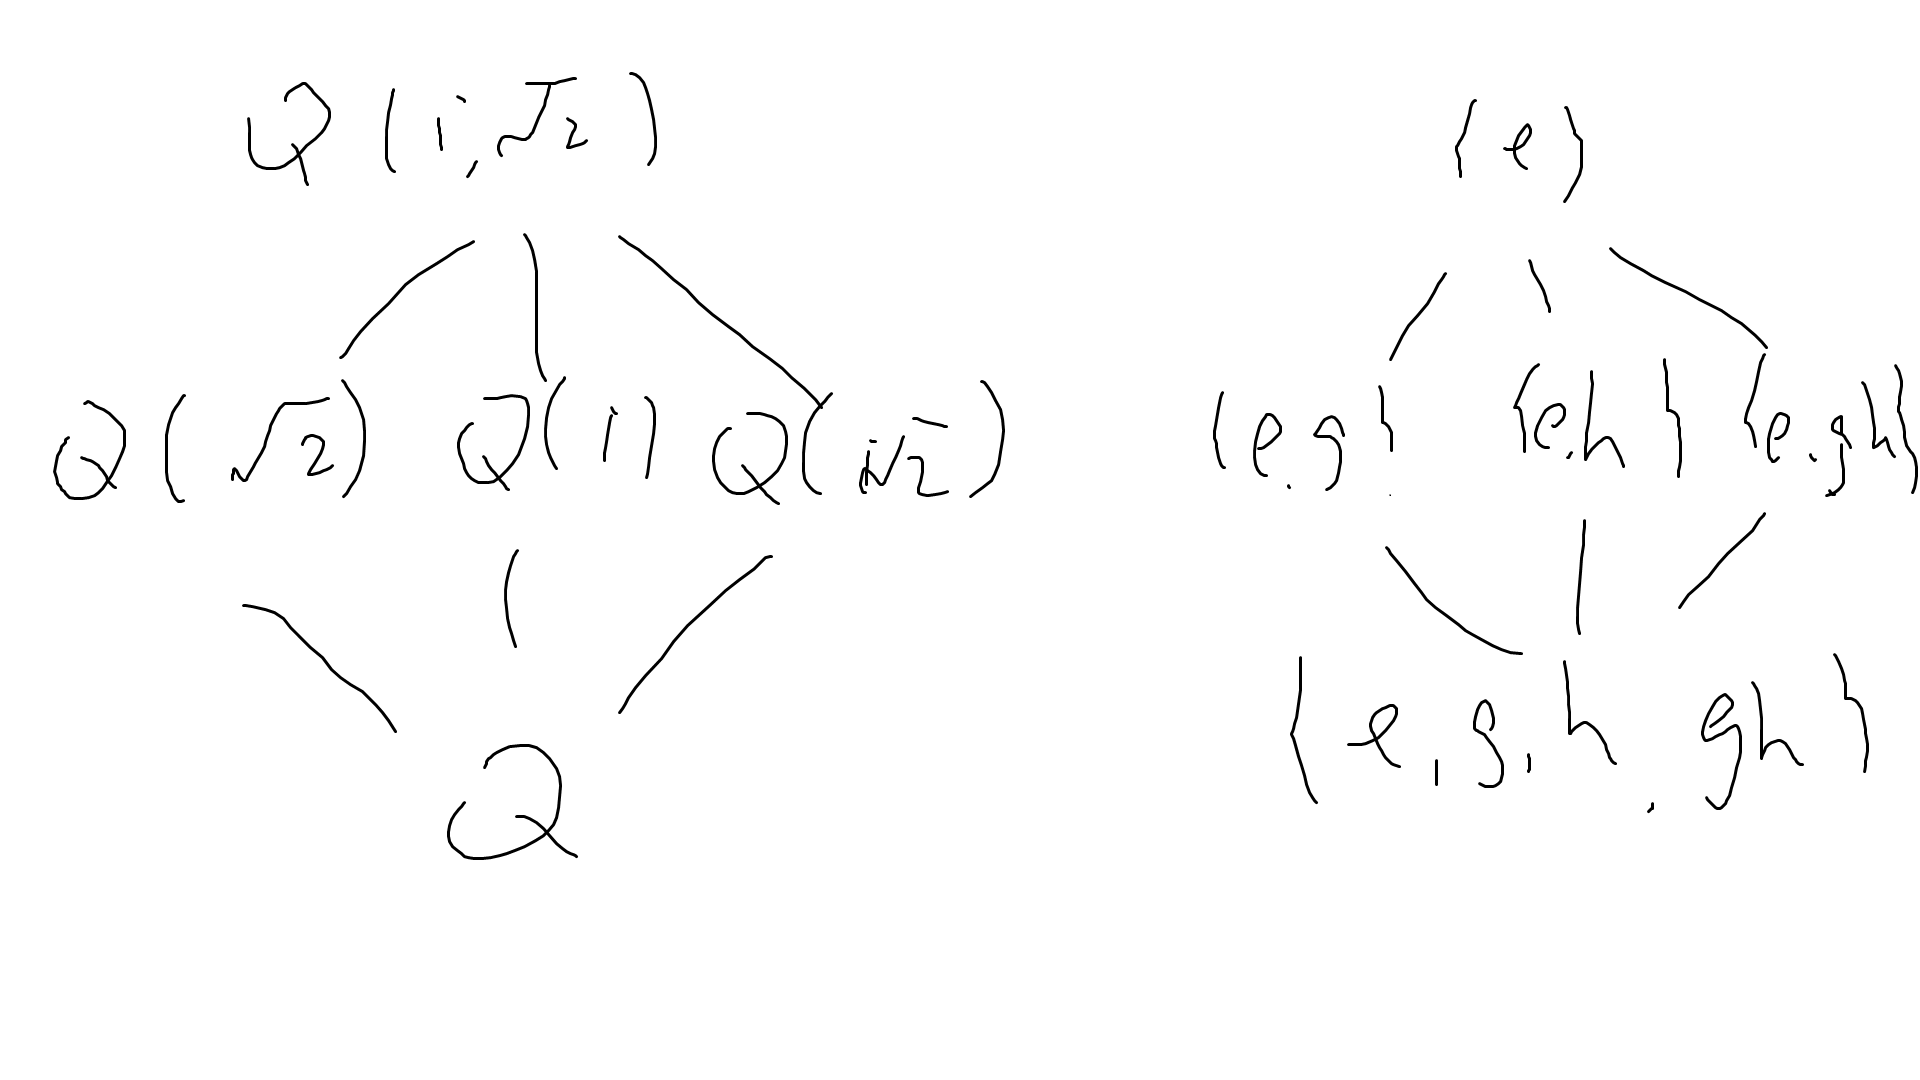
\includegraphics[scale=0.4]{image/GT_01.png}

The recipe for producing an intermediate subfield from a subgroup is to take the elements of $\Q(i,\sqrt{2})$ which are fixed by all elements of the subgroup, e.g. $\Q(i\sqrt{2})$ is the field of elements fixed by both $e$ and $gh$.

This correspondence doesn't always work for all finite field extensions. It works for \emph{Galois extensions}.

In the correspondence, normal extensions correspond to normal subgroups. In the above example, all subgroups are normal and the extensions are normal.

We'll also prove the Primitive Element Theorem, which in the context of finite extensions of $\Q$, tells us that they are necessarily of the form $\Q(\alpha)$ for some $\alpha$, e.g. $\Q(i,\sqrt{2})$ (or $\Q(i+\sqrt{2})$).

Now let's review some material from GRM:

\begin{defi}
Suppose $K \leq L$ is a field extension. Take $\alpha \in L$. We define $I_\alpha = \{f \in K[t] : f(\alpha) = 0\}$, i.e. all the polynomials on $K$ with $\alpha$ a root. $\alpha$ is \emph{algebraic} over $K$ if $I_\alpha \neq \{0\}$. Otherwise, $\alpha$ is \emph{transcendental}.

We say $L$ is algebraic over $K$ if $\alpha$ is algebraic over $K$ for all $\alpha \in L$.
\end{defi}

\begin{rem}
\begin{equation*}
\begin{aligned}
I_\alpha = \ker\ \left(
\begin{array}{ll}
K[t] &\to L\\
f(t) &\to f(\alpha)\\
\end{array}
\right)
\end{aligned}
\end{equation*}
i.e. the set of polynomials in $K[t]$ that have $\alpha$ as a root, is an ideal of $K[t]$.
\end{rem}

\begin{eg}
$\sqrt{2}$ is algebraic over $\Q$. $\pi$ is transcendental over $\Q$.
\end{eg}

\begin{lemma}(1.5)\\
Let $K \leq L$ be a finite field extension. Then $L$ is algebraic over $K$.
\begin{proof}
Let $|L:K| = n$. Take $\alpha \in L$. Consider $1,\alpha,\alpha^2,...,\alpha^n$. These must be linearly dependent in the $n$-dimensional $K$-vector space $L$. Therefore $\sum_0^n \lambda_i \alpha^i=0$ for some $\lambda_i \in K$ not all zero. Then $\alpha$ is a root of $f(t) = \sum_0^n \lambda_i t^i$, i.e. algebraic over $K$.
\end{proof}
\end{lemma}

\begin{defi}(1.6)\\
The non-zero ideal $I_\alpha$ (where $\alpha$ is algebraic over $K$) is principal, since $K[t]$ is a principal ideal domain ($K$ is a field, so $K[t]$ is in fact a ED). So let $I_\alpha = (f_\alpha(t))$ and $f_\alpha(t)$ can be assumed to be monic. Such a monic $f_\alpha(t)$ is the \emph{minimal polynomial of $\alpha$ over $K$}.
\end{defi}

\begin{rem}
Multiplication by $\alpha$ within the field $L$ gives a $K$-linear map $L \to L$, an automorphism (if $\alpha \neq 0$). In GRM we proved that the minimal polynomial of a linear map is unique.
\end{rem}

\begin{eg}
The minimal polynomial of $\sqrt{2}$ over $\Q$ is $t^2-2$, and is $t-\sqrt{2}$ over $\R$.
\end{eg}

\begin{lemma}(1.7)\\
Suppose $K \leq L$ is a field extension, and $\alpha \in L$ is algebraic over $K$. Then the minimal polynomial $f_\alpha(t)$ of $\alpha$ over $K$ is irreducible in $K[t]$. As a result, $I_\alpha$ is a prime ideal.
\begin{proof}
Suppose $f_\alpha(t) = p(t) q(t)$. We must show that either $p(t)$ or $q(t)$ is a unit in $K[t]$. Note that 
\begin{equation*}
\begin{aligned}
0 = f_\alpha(\alpha) = p(\alpha)q(\alpha)
\end{aligned}
\end{equation*}
WLOG assume $p(\alpha)=0$. Then $p(t) \in I_\alpha$, i.e. $p(t) = f_\alpha(t) \cdot r(t)$ since $I_\alpha = (f_\alpha(t))$. So $f_\alpha(t) = f_\alpha(t) r(t) q(t)$, i.e. $r(t) q(t) = 1$, hence $q(t)$ is a unit of $K[t]$. So $f_\alpha(t)$ is irreducible.

Recall from GRM that irreducible elements of $K[t]$ are prime ($K[t]$ is PID), and generate prime ideals of $K[t]$. So $I_\alpha$ is a prime ideal.
\end{proof}
\end{lemma}

\begin{defi} (1.8)\\
Suppose $K \leq L$ is a field extension, and $\alpha \in L$. $K(\alpha)$ is the smallest subfield of $L$ that contains both $K$ and $\alpha$, called the field generated by $K$ and $\alpha$. We say that $L$ is a \emph{simple extension} if $L=K(\beta)$ for some $\beta \in L$.
\end{defi}

Note that the previous Primitive Element Theorem can be restated as: any finite extension of $Q$ is a simple extension over $\Q$.

Also, given $\alpha_1,...,\alpha_n \in L$, $K \leq L$, we call $K(\alpha_1,...,\alpha_n)$ the smallest intermediate field containing $\alpha_1,...,\alpha_n$. It is the field generated by $K$ and $\alpha_1,...,\alpha_n$. 

On the other hand we'll prove that $K[\alpha]$, the image of the map $K[t] \to L$ by $f(t) \to f(\alpha)$, is the \emph{ring} generated by $K$ and $\alpha$ (for $\alpha \in L$).

\begin{thm} (1.9)\\
Suppose $K \leq L$ is a field extension, $\alpha \in L$ is algebraic over $K$. Then\\
(i) $K(\alpha) = K[\alpha]$;\\
(ii) $|K(\alpha):K| = \deg f_\alpha (t)$ where $f_\alpha(t)$ is the minimal polynomial of $\alpha$ over $K$.
\begin{proof}
(i) Clearly $K[\alpha] \leq K(\alpha)$. We need to show that if $0 \neq \beta \in K[\alpha]$, then it is a unit in $K[\alpha]$, so $K[\alpha] $  is a field.\\
For every $\beta$ we have $\beta=g(\alpha)$ for some $g(t) \in K[t]$. Since $\beta = g(\alpha) \neq 0$, $g(t) \not\in I_\alpha = (f_\alpha(t))$. Thus $f_\alpha(t) \nmid g(t)$. From theorem 1.7, $f_\alpha(t)$ is irreducible. From GRM, since $K[t]$ is a PID, we know there exist $r(t),s(t) \in K[t]$ with $r(t) f_\alpha(t) + s(t) g(t) = 1$ in $K[t]$. Hence $s(\alpha) g(\alpha) = 1$ in $K[\alpha]$. So $\beta = g(\alpha)$ is a unit as required.

(ii) Let $n = \deg f_\alpha(t)$. We'll show that $\{1,\alpha,...,\alpha^{n-1}\}$ is a $K$-vector space basis of $K[\alpha]$.\\
If $f_\alpha(t) = t^n + a_{n-1}t^{n-1}+...+a_0$ with $a_i \in K$, then $\alpha^n = -a_{n-1}\alpha^{n-1} -...-a_0$. This implies that $\alpha^n$ is a linear combination of $\{1,...,\alpha^{n-1}\}$.\\
An easy induction shows that $\alpha^m$ for $m \geq n$ is likewise a linear combination of $\{1,\alpha,...,\alpha^{n-1}\}$. Thus the above set spans $K[\alpha]$.\\
Suppose $\lambda_{n-1}\alpha^{n-1}+...+\lambda_0=0$. Let $g(t) = \lambda_{n-1}t^{n-1}+...+\lambda_0$. Since $g(\alpha)=0$, we have $g(t) \in I_\alpha = (f_\alpha(t))$. So $g(t) = 0$ or $f_\alpha(t) \mid g(t)$. The latter is not possible because $\deg f_\alpha(t) > \deg g(t) = n-1$. So $g(t)=0 in K[t]$, and all the $\lambda_i$ must then be zero.
\end{proof}
\end{thm}

\begin{coro} (1.10)\\
If $K \leq L$ is a field extension and $\alpha \in L$, then $\alpha$ is algebraic over $K$ $\iff$ $K \leq K(\alpha)$ is finite.
\begin{proof}
The forward direction is given by (1.9), $|K(\alpha):K| = \deg f_\alpha(t) < \infty$. The backward is given by (1.5).
\end{proof}
\end{coro}

\begin{coro} (1.11)\\
Let $K \leq L$ be a field extension with $|L:K|=n$. Let $\alpha \in L$. Then $\deg f_\alpha(t) | n$.
\begin{proof}
Use the Tower Law (1.3) on $K \leq K(\alpha) \leq L$, we deduce that $|K(\alpha) : K| $ divdes $|L:K|$. (1.9) says that $\deg f_\alpha(t) = |K(\alpha):K|$.
\end{proof}
\end{coro}

\subsection{Constructibility problems}
Now let's digress on some constructibility problems. Assume we're given a set $P_0$ of points in $\R^2$. A ruler operation is to draw a straight line through any two points in $P_0$, and a compass operation is to draw a circle with a centre being a point in $P_0$ and radius equal to tidtance between a pair of points in $P_0$.

\begin{defi} (1.12)\\
The points of intersection of any two distinct lines or circles drawn using those operations are constructible in one step from $P_0$.

A point $\mathbf{r} \in \R^2$ is constructible from $P_0$ if there is a finite sequence $\mathbf{r}_1,...,\mathbf{r}_n = \mathbf{r}$ Such that $r_i$ is constructible in one step from $P \cup \{r_1,...,r_{i-1}\}$.
\end{defi}

An easy exercise is to construct the midpoint of a line between two points.

Now let $K_0$ be the subfield of $\R$ generated by $\Q$ and the coordinates of the points in $P_0$. Let $\mathbf{r}_i = (x_i,y_i)$. Set $K_i = K_{i-1} (x_i,y_i)$. Thus $K_0 \leq K_1 \leq ... \leq K_m \leq \R$.

\begin{lemma} (1.13)\\
$x_i$, $y_i$ are both roots in $K_i$ of quadratic polynomials in $K_{i-1}[t]$.
\begin{proof}
We have 3 cases of intersections: line meets line, line meets circle, circle meets circle. We can just consider the equations of lines/circles and solve a system of equation for each case of intersection, which in all three cases are at most quadratic equations.
\end{proof}
\end{lemma}

\begin{thm} (1.14)\\
If $\mathbf{r} = (x,y)$ is a constructible point from set $P_0$ of points in $\R^2$, and if $K_0$ is the subfield of $\R$ generated by $\Q$ and the coordinates of the points in $P_0$, then the degrees $|K_0(x):K_0|$ and $|K_0(y):K_0|$ are both powers of $2$.
\begin{proof}
We continue with the previous notation, $K_i = K_{i-1} (x_i,y_i)$. By tower law,
\begin{equation*}
\begin{aligned}
|K_i:K_{i-1}| = |K_{i-1}(x,y):K_{i-1}(x)| |K_{i-1}(x) : K_{i-1}|
\end{aligned}
\end{equation*}
But (1.13) tells us that $|K_{i-1}(x):K_{i-1}|$ is $1$ or $2$ using degree of extension $=$ degree of minimal polynomial of $x$ over $K_{i-1}$. Similarly $y$ satisfies a quadratic polynomial over $K_{i-1}$ and hence over $K_{i-1}(x)$. So $|K_{i-1}(x,y):K_{i-1}(x)|$ is $1$ or $2$.

So $|K_i:K_{i-1}|$ is 1,2 or 4 (but $4$ doesn't happen -- that doesn't matter anyway in this proof). Then we just use tower law recursively. Now if $\mathbf{r}=(x,y)$ is constructible from $P_0$ then we can write $x,y \in K_n$ and $K_0 \leq K_0(x) \leq K_n$ and $K_0 \leq K_0(y) \leq K_n$. Then again by tower law we know the two indexes must be some powers of $2$.
\end{proof}
\end{thm}

That is a nice theorem to determine constructibility, but to actually use it we need to be reasonable expert at working out minimal polynomials. Recall from GRM that

\begin{thm} (1.15, Gauss' lemma)\\
Let $f(t)$ be a primitive integral polynomial. Then $f(t)$ is irreducible in $\Q[t]$ iff $f(t)$ is irreducible in $\Z[t]$.
\end{thm}
Another useful tool is
\begin{thm} (1.16, Eisenstein's criterion)\\
Let $f(t) = a_n t^n + a_{n-1} t^{n-1} + ... + a_0 \in \Z[t]$. Suppose there is a prime $p$ such that\\
(1) $p \nmid a_n$;\\
(2) $p \mid a_i$ for $i=0,...,n-1$;\\
(3) $p^2 \nmid a_0$.
Then $f(t)$ is irreducible in $\Z[t]$.
\end{thm}

Another method is to consider an integral polynomial $f(t) \pmod p$. If $f(t)$ is reducible in $\Z[t]$ then it is reducible in $\Z/p\Z$. So if we find a prime $p$ such that $f(t) \pmod p$ is irreducible, then $f(t)$ must be irreducible in $\Z[t]$.

To see how this work, we prove that $t^3+t+1$ is irreducible. Consider $\Z/2\Z$, if it were irreducible it would have a linear factor and the polynomial would have a root; but neither $0$ nor $1$ is a root. So $t^3+t+1$ is not reducible mod $2$, so not reducible in $\Z[t]$ (and $\Q[t]$) either.

However, on later example we'll see an example that is irreducible in $\Z[t]$ but is reducible mod $p$ for all primes $p$. So this method is not sufficient in all cases.

\begin{thm} (1.17)\\
The cube cannot be duplicated by ruler and compasses.
\begin{proof}
The problem amounts to whether given a unit distance, one can construct points distanced $\alpha=\sqrt[3]{2}$ apart, i.e. starting with $P_0=\{(0,0),(1,0)\}$, can we produce $(\alpha,0)$? The answer is NO -- if we could then we need $|\Q(\alpha):\Q|$ to be a power of $2$, but $|\Q(\alpha):\Q|=\deg f_\alpha(t) = 3$ as $f_\alpha(t) = t^3-2$ and we know that that is not reducible (using Eisenstein's with $p=2$).
\end{proof}
\end{thm}

\begin{thm} (1.18)\\
The circle cannot be squared using ruler and compasses.
\begin{proof}
Similarly, the problem becomes starting with $(0,0)$ and $(1,0)$, can we construct $(\sqrt{\pi},0)$. But we know $\pi$ is transcendental over $\Q$ (by Lindermann -- not proved here).
\end{proof}
\end{thm}

\subsection{Field extensions}
Now we return to our theory development.

\begin{lemma} (1.19)\\
Let $K \leq L$ be a field extension. Then\\
(i) $\alpha_1,...,\alpha_n \in L$ are algebraic over $K$ if and only if $K \leq K(\alpha_1,...,\alpha_n)$ is a finite extension.\\
(ii) If $K \leq M \leq L$ such that $K \leq M$ is finite, then there exists $\alpha_1,...,\alpha_n \in L$ such that $K(\alpha_1,...,\alpha_n) = M$.\\
Note that $L$ isn't really relevant in the second part.
\begin{proof}
(i) By (1.10), $\alpha$ is algebraic over $K$ if and only if $K \leq K(\alpha)$ is a finite field extension. $\alpha_i$ is algebraic over $K$, hence algebraic over $K(\alpha_1,...,\alpha_{i-1})$. So $|K(\alpha_1,...,\alpha_i):K(\alpha_1,...,\alpha_{i-1})|$ is finite. By tower law applied to $K \leq K(\alpha_1) \leq K(\alpha_1,\alpha_2) \leq ... \leq K(\alpha_1,...,\alpha_n)$, we get $|K(\alpha_1,...,\alpha_n):K|$ is finite.

Conversely, consider $K \leq K(\alpha_1)\leq K(\alpha_1,...,\alpha_n)$. Then the tower law says that if $|K(\alpha_1,...,\alpha_n) :K|$ is finite then $|K(\alpha_i):K|$ is also finite for any $i$, i.e. $\alpha_i$ is algebraic.

(ii) If $|M:K|=n$, then $M$ is an $n$-dimensional $K$-vector space by definition. So there exists a $K$-basis $\alpha_1,...,\alpha_n$ of $M$. Then $K(\alpha_1,...,\alpha_n) \leq M$. However, element of $M$ is a $K$-linear combination of $\alpha_1,...,\alpha_n$, so we also have $M \leq K(\alpha_1,...,\alpha_n)$. So they are equal.
\end{proof}
\end{lemma}

\begin{defi} (1.20)\\
Suppose $K \leq L$, $K \leq L'$ are fields extensions. A $K$-homomorphism: $\phi: L \to L'$ is a ring homomorphism such that $\phi|_K = id$.
\end{defi}

We'll occasionally use the notation $Hom_K(L,L') = \{K$-homomorphisms $L \to L'\}$.

A $K$-homomorphism $\phi:L \to L'$ is a $K$-isomorphism if it is a ring isomorphism.

We have another notation, $\Aut_K(L) = \{K-$isomorphisms $L \to L\}$ which is a group.

\begin{lemma} (1.21)\\
Suppose $K \leq L$, $K \leq L'$ are field extensions. Then \\
(i) Any $K$-homomorphism $\phi:L \to L'$ is injective, and $K \leq \phi(L)$ is a field extension;\\
(ii) If $|L:K| = |L':K|$ is finite, then any $K$-homomorphism is actually a $K$-isomorphism.
\begin{proof}
(i) $L$ is a field, so $\ker(\phi)$ is an ideal of $L$. Note that $1 \to 1$ by $\phi$, so $\ker \phi$ can't be the whole of $L$. So $\ker\phi = \{0\}$, i.e. $\phi(L)$ is a field and $K \leq \phi(L)$ is a field extension.

(ii) $\phi$ is an injective $K$-linear map, and so $|\phi(L):K| = |L:K|$ considering dimensions of $K$-vector spaces. As a result, $\phi(L) = L'$, i.e. $\phi$ is an isomorphism.\\
In particular, if $L=L'$, then $\phi$ is an $K$-automorphism of $L$.
\end{proof}
\end{lemma}

We introduce another notation: If $K \leq L$ is a field extension, and if $f(t) \in K[t]$, we denote the set of roots of $f$ in $L$ by $Root_f (L)$.

\begin{defi} (1.22)\\
Let $K \leq L$ be a field extension, and $f(t) \in K[t]$. We say $f$ \emph{splits over $L$} if $f(t) = a(t-\alpha_1)...(t-\alpha_n)$, where $a \in K$, $\alpha_1,...,\alpha_n \in L$. We say $L$ is a \emph{spltting field} for $f$ over $K$ if $L = K(\alpha_1,...,\alpha_n)$.
\end{defi}

\begin{rem}
This is equivalent to saying that $L$ is a splitting field for $f$ over $K$ if and only if:\\
(i) $f$ splits over $K$;\\
(ii) if $K \leq M \leq L$ and $f$ splits over $M$ then $M = L$ (minimality).
\end{rem}

\begin{eg}
(1) $f(t) = t^3-2$ over $\Q$. $\Q(\sqrt[3]{2})$ is not a splitting field for $f$ over $\Q$, but $\Q(\sqrt[3]{2},\omega \sqrt[3]{2},\omega^2 \sqrt[3]{2})$ is a splitting field over $Q$, where $\omega$ is the primitive cube root of unity. Note that the above field is equal to $\Q(\sqrt[3]{2},\omega)$.\\
Note that $\Q(\sqrt[3]{2})$ is degree $3$ over $\Q$, but $\Q(\omega)$ is only degree 2. Also $|\Q(\sqrt[3]{2},\omega):\Q(\omega)|\leq 3$ and $|\Q(\sqrt[3]{2},\omega) : \Q(\sqrt[3]{2})| \leq 2$. Then use the tower law and we get $2 \mid |\Q(\sqrt[3]{2},\omega):\Q|$, and $3$ also divides it. So $\Q(\sqrt[3]{2},\omega)$ must be at least degree 6. So the two previous inequalities actually have their equal signs hold.

(2) $f(t) = (t^2-3)(t^3-1)$. Splitting field for $f$ over $\Q$ is $\Q(\sqrt{3},-\sqrt{3},\omega,\omega^2,1) = \Q(\sqrt{3},\omega) = \Q(\sqrt{3},i)$ since we know $\omega = \frac{-1+\sqrt{3}}{2}$.

(3) $t^2-3$ and $t^2-2t-2$ both have the same splitting field $\Q(\sqrt{3})$ over $\Q$.

(4) $f(t) = t^2+t+1$ in $\F_2[t]$ (where $\F_2 =$ field of $2$ elements $0,1 = \Z / 2\Z$). $f(t)$ is irreducible over $\F_2$ since it has no roots in $\F_2$ and hence no linear factors $\F_2[t]$. So $\F_2[t] / (t^2+t+1)$ is a field.

Now set $\alpha = t+(t^2+t+1) \in \F_2[t] / (t^2+t+1)$. Then $\F_2[t] / (t^2+t+1) = \F_2(\alpha)$. The elements are $0,1,\alpha,\alpha+1$. $f(t) =t^2+t+1$ splits over $\F_2(\alpha)$  noting that $\alpha^2 = \alpha+1$. Now $f(t) = (t-\alpha)(t-1-\alpha)$. Thus $\F_2(\alpha)$ is splitting field for $f$ over $\F_2$.
\end{eg}

We use this construction to produce splitting field in general.

\begin{thm} (1.23, Existence of splitting fields)\\
Let $K$ be a field, and $f(t) \in K[t]$. Then there exists a splitting field for $f$ over $K$.
\begin{proof}
If $\deg f = 0$, then $K$ itself is the splitting field.\\
Now let $\deg f >0$ and pick an irreducible factor $g(t)$ of $f(t)$ in $K[t]$. Note $K \leq K[t] / (g(t))$ is a field extension.\\
Now take $\alpha_1 = t+(g(t)) \in K[t] / (g(t))$. Then $K[t] / (g(t)) = K(\alpha_1)$ and $g(\alpha_1) = 0$ in $K(\alpha_1)$; therefore $f(\alpha_1) = 0$ in $K(\alpha_1)$, and we can write $f(t) = (t-\alpha_1) h(t)$ in $K(\alpha_1)[t]$. Repeat, noting that $\deg h(t) < \deg f(t)$, and we get $f(t) = a(t-\alpha_1) (t-\alpha_2) ... (t-\alpha_n)$ where $a$ is a constant, which is in $K$ (consider top coefficient).\\
Thus we have a factorization of $f(t)$ in $K(\alpha_1,...,\alpha_n)[t]$, i.e. $K(\alpha_1,...,\alpha_n)$ is a splitting field for $f$ over $K$.
\end{proof}
\end{thm}

\begin{thm} (1.24, Uniqueness of splitting fields)\\
If $K$ is a field and $f(t) \in K[t]$, then the splitting field for $f$ over $K$ is unique up to $K$-isomorphisms.
\begin{proof}
Suppose $L$ and $L'$ are both splitting fields for polynomial $f(t) \in K[t]$ over $K$. We need to show that there is a $K$-isomorphism $L \to L'$. Suppose $K \leq M \leq L$ and $\exists K \leq M' \leq L'$ and a $K$-isomorphism $\psi: M \to M'$; clearly we can always take $M=K$, so such $M$ always exists. Now we pick $M$ so that $|M:K|$ is maximal among all such $M,M',\psi$. We must show $M=L$ and $M'=L'$. Note that if $M=L$, then $f(t)$ splits over $L$ then $f(t)$ splits over $M$, i.e. $f(t) = a(t-\alpha_1)...(t-\alpha_m)$ in $M[t]$. Now apply $\psi$, we got an induced map $M[t] \to M'[t]$, and $f(t) \to \psi f(t) = \psi(a)(t-\psi(\alpha_1))...(t-\psi(\alpha_m))$, thus $f(t)$ splits over $\psi(M) = M'$. But $L'$ is a splitting field, and $M' \leq L'$; but a splitting field is the minimal field extension that $f$ splits; so $M'=L'$.

Otherwise, if $M \neq L$, we want to get a contradiction of maximality of $M$. Since $M < L$, there is a root $\alpha$ of $f(t) \in L$ that is not in $M$. Now factorize $f(t) = g(t) h(t)$ in $M[t]$ so that $g(t)$ is irreducible in $M[t]$ and $g(\alpha)=0$ in $L$. Then there exists a $K$-homomorphism $M[t]/(g(t)) \to L$ by $t+(g(t)) \to \alpha$. The image of this is $M(\alpha)$, the $K$-isomorphism $M[t] \to M'[t]$ induced by $\psi$ maps $g(t)\in M[t]$ to some $\gamma(t) \in M'[t]$. Now $f(t) = g(t)h(t)$ in $M[t]$ is mapped to $f(t) = \gamma(t) \delta(t)$ in $M'[t]$. We now have a field extension $M' \leq M'[t] / (\gamma(t))$, and there exists a $M'$-homomorphism $M'[t]/(\gamma(t)) \in L'$ by picking a root $\alpha'$ of $\gamma(t)$ in $L'$, sending $t+(\gamma(t)) \to \alpha'$. However $\gamma(t) |f(t)$ in $M'[t]$, hence in $L'[t]$. As a result, this root $\alpha'$ is also a root of $f(t)$ in $L'$. The $M'$-homomorphism gives a $K$-isomorphism $M'[t] / (\gamma(t)) \to M'(\alpha')$, and so we have a $K$-isomorphism $M(\alpha) \to M'(\alpha')$. This contradicts the maximality of $M$ and $M'$.
\end{proof}
\end{thm}

\begin{defi} (1.25)\\
An algebraic field extension $K \leq L$ is \emph{normal} if for every $\alpha \in L$, the minimal polynomial $f_\alpha(t)$ of $\alpha$ over $K$ splits over $L$.
\end{defi}

\begin{thm} (1.26)\\
Let $K \leq L$ be a finite field extension. Then $K \leq L$ is normal $\iff$ $L$ is the splitting field for some $f(t) \in K[t]$.
\begin{proof}
This proof will be presented later.
\end{proof}
\end{thm}

\begin{eg} (1.27)\\
Let $\F$ be a finite field, with $|\F| = m$. We know $\F$ has characteristic $p$ for some prime $p$, and $\F_p \leq \F$. Therefore $m=p^r$ for some $r$. The non-zero elements from the multiplicative group, of order $m-1=n$, say. Also they satisfy $t^n-1$, i.e. they are roots of $t^n-1$. So $t^n-1 = (t-\alpha_1)...(t-\alpha_n)$ where $\alpha_1,...,\alpha_n$ are the non-zero elements of $\F$. Thus $\F$ is the splitting field for $t^n-1$ over $\F_p$. By (1.24) we have uniqueness of splitting fields, so any other field with $m$ elements is $\F_p$-isomorphic to $\F$. (Note that we haven't shown that there exists such a $\F$).
\end{eg}

\begin{thm} (1.28)\\
Let $G$ be a finite subgroup of the multiplicative group of a field $K$. Then $G$ is cyclic. In particular, the multiplicative group of a finite field is cyclic.
\begin{proof}
Let $|G|=n$. By structure theorem of finite abelian groups, we have
\begin{equation*}
\begin{aligned}
G \cong C_{q_1^{m_1}} \times C_{q_2^{m_2}} \times ... \times C_{q_r^{m_r}}
\end{aligned}
\end{equation*}
with $q_i$ prime, but not necessarily distinct. However, if we have $q=q_i = q_j$ for some $i \neq j$, there are at least $q^2$ distinct solutions of $t^q-1=0$ in $K$, since $C_q \times C_q$ is isomorphic to a subgroup of $G$. However in a field (even in an integral domain), we know a polynomial of degree $q$ has at most $q$ roots. So the $q_i$ must be distinct and hence $G$ is actually cyclic, generated by $(g_1,...,g_r)$ where $g_i$ generates $C_{q_i^{m_i}}$.
\end{proof}
\end{thm}

\newpage

\section{Separable, Normal and Galois Extensions}

\subsection{Separable extensions}

\begin{defi} (2.1)\\
Let $K$ be a field and $f(t) \in K[t]$. Suppose $f(t)$ is irreducible in $K[t]$, and $L$ is a splitting field of $f(t)$ over $K$. Then $f(t)$ is \emph{separable over $K$} if $f(t)$ has no repeated roots in $L$. For general $f(t)$, we say $f(t)$ is \emph{separable over $K$} if every irreducible factor in $K[t]$ is separable over $K$. All constant polynomials are deemed to be separable.
\end{defi}

\begin{defi} (2.2)\\
If $K$ is a field, then formal differentiation $D:K[t] \to K[t]$ is a $K$-linear map with $D(t^n) = nt^{n-1}$. We denote $D(f(t))$ by $f'(t)$.
\end{defi}

\begin{lemma} (2.3)\\
Let $K$ be a field, $f(t),g(t) \in K[t]$. Then
\begin{equation*}
\begin{aligned}
D(f(t)g(t)) = f'(t)g(t)+f(t)g'(t)
\end{aligned}
\end{equation*}
and if $f(t) \neq 0$, then $f(t)$ has a repeated root in a splitting field if and only if $f(t)$ and $f'(t)$ have a common irreducible factor in $K[t]$.
\begin{proof}
(a) $D$ is a $K$-linear map and so we only need to checo for $f(t) = t^n$ and $g(t) = t^m$. (check)

(b) Let $\alpha$ be a repeated root in a splitting field $L$. Then $f(t) = (t-\alpha)^2g(t)$ in $L[t]$, hence $f'(t) = (t-\alpha)^2 g'(t) + 2(t-\alpha)g(t)$ and so $f'(\alpha) = 0$. Therefore the minimal polynomial $f_\alpha(t)$ of $\alpha$ in $K[t]$ divides both $f(t)$ and $f'(t)$, and thus $f_\alpha(t)$ is a common irreducible factor of $f(t)$ and $f'(t)$. Conversely, let $h(t)$ be a common irreducible factor of $f(t)$ and $f'(t)$ in $K[t]$. Pick a root $\alpha$ in $L$ of $h(t)$, so $f(\alpha) = 0 = f'(\alpha)$. Thus $f(t) = (t-\alpha) g(t)$ in $L[t]$, and $f'(t) = (t-\alpha) g'(t) + g(t)$. Since $f'(\alpha) =0 $, we have $(t-\alpha) | f'(t)$, so $(t-\alpha)|g(t)$. Hence we have $(t-\alpha)^2 | f(t)$.
\end{proof}
\end{lemma}

\begin{coro} (2.4)\\
If $K$ is a field and $f(t) \in K[t]$ is irreducible,\\
(i) If $char(K) = 0$ then $f(t)$ is separable over $K$;\\
(ii) If $char(K)=p>0$ then $f(t)$ is not separable if and only if $f(t) \in K[t^p]$.
\begin{proof}
By (2.3), $f(t)$ is not separable if and only if $f(t)$ and $f'(t)$ has a common irreducible factor. But $f(t)$ is not irreducible, the only possible factor is $f(t)$ itself, i.e. $f(t) | f'(t)$, i.e. $f'(t) =0$ since it has a smaller degree. But then if $f(t) = a_n t^n + ... + a_0$, then $f'(t) = na_n t^{n-1}+...+a_1$, thus $f'(t) = 0 \iff ia_i=0 \forall i \geq 1$. So \\
(i) $char(K) = 0$, so $f'(t) \neq 0$ for non-constant polynomial $f(t)$. So $f(t)$ is separable over $K$.\\
(ii) If $char(K) = p > 0$, then if $f'(t) = 0$ we have $ia_i = 0 \forall i>0$, i.e. $f(t)$ is not separable $\iff$ $f(t) \in K[t^p]$.
\end{proof}
\end{coro}

\begin{defi}(2.5)\\
If $K \leq L$ is a field extension, we say $\alpha \in L$ is separable over $K$ if its minimal polynomial is separable over $K$. $L$ is separable over $K$ if all elements of $L$ are separable over $K$. If the minimal polynomial of $\alpha$ is $f_\alpha(t) = (t-\alpha)^n = t^n - \alpha^n$ where $n$ is a power of $p$ ($=char(K)$), we say $\alpha$ is \emph{purely inseparable} over $K$.
\end{defi}

\begin{eg} (2.6)\\
(1) Let $\Q \subseteq L$ be an algebraic field extension. Then $L$ is separable over $\Q$.\\
(2) Let $L = \F_p(X)$, the rational functions in $X$ over $\F_p$, and $K = \F_p (X^p)$ be a subfield. Then $K \leq L$ is not separable: observe that if $f(t) = t^p - X^p \in K[t]$. Then $f'(t) = 0$. But $t^p-X^p = (t-X)^p$ in $L[t]$. However, $f(t)$ is irreducible in $K[t]$: suppose we have a factorization $f(t) = g(t)h(t)$ in $K[t]$ and hence in $L[t]$, so we get $g(t) = (t-X)^r$ for some $0 \leq r < p$ if the factorisation is non-trivial. But this would mean $X^r$ was in $K$. However (again), $\exists$ integers $a,b$ s.t. $ar+bp=1$, so $(X^r)^a (X^p)^b \in K$, i.e. $X \in K$. Thus we'd have $X = u(X^p)/v(X^p)$, contradiction.\\
Thus $f(t) = t^p -X^p$ is the minimal polynomial of $X$ over $K$. Thus $X$ is purely inseparable over $K$, and $K \leq l$ is not separable.\\
(3) Let $\F$ be a finite field with $|\F| = m$, a power of $p = char(\F)$, and $f(t) = t^n - 1$ where $n=m-1$. We know this is separable over $\F_p$ since we saw that $f(t)$ has distinct linear factors in $F[t]$.
\end{eg}

\begin{rem}
It's useful to have an alternative approach to separability of field extensions without having to check separability of minimal polynomials for all elements of the larger field. This is where we start thinking about $K$-homomorphisms.
\end{rem}

\begin{lemma} (2.6)\\
Let $M = K(\alpha)$ for $\alpha$ algebraic over $K$, and let $f_\alpha(t)$ be the minimal polynomial of $\alpha$ over $K$. For any field extension $K \leq L$, then the number of $K$-homomorphisms of $M$ to $L$ is equal to the number of distinct roots of $f_\alpha(t)$ in $L$. Thus this number $\leq \deg f_\alpha(t) = |K(\alpha):K| = |M:K|$.
\begin{proof}
We saw in (1.21) that any $K$-homomorphism $M$ to $L$ is injective, $K(\alpha) \cong K[t]/(f_\alpha(t))$. For any root $\beta$ of $f_\alpha(t)$ in $L$, we can define a $K$-homomorphism $K[t]/(f_\alpha(t)) \to L$ that sends $t+(f_\alpha(t)) \to \beta$. Thus we get a $K$-homomorphism $M \to L$. Conversely, for any $K$-homomorphism $\phi:M \to L$, the image $\phi(\alpha)$ must satisfy $f_\alpha(\phi(\alpha)) = 0$. These processes are inverse to each other,
\end{proof}
\end{lemma}

(missing lecture 8)

\begin{thm} (2.17, Theorem of the primitive element)\\
Any finite separable extension $K \leq M$ is a simple extension, i.e. $M = K(\alpha)$ for some $\alpha$, called the \emph{primitive element}.

\begin{proof}
If $K$ is a finite field, then $M$ is also finite. So we can take $K$ to be a generator of the multiplicative group of $M$ (which is cyclic).

Now assume $K$ is an infinite field. Since $K \leq M$ is a finite extension, $M = K(\alpha_1,...,\alpha_n)$ for some $\alpha_i$. It's enough to show that any field $M=K(\alpha,\beta)$ with $\beta$ separable over $K$ is of the form $K(\gamma)$. Take $f(t)$ and $g(t)$ to be the minimal polynomials of $\alpha$ and $\beta$ over $K$. Let $L$ be the splitting field for $f(t) g(t)$ over $K(\alpha,beta)$. The distinct zeros of $f(t)$ in $L$ are $\alpha = \alpha_1,...,\alpha_a$, and of $g(t)$ are $\beta = \beta_1,...,\beta_b$. By separability we know $b = \deg g(t)$. Choose $\lambda \in K$ such that all $\alpha_i + \lambda \beta_j$ are distinct (this is possible since $K$ is infinite). Now we set $\gamma = \alpha_\lambda\beta$ (remember $\alpha$ is $\alpha_1$ and $\beta$ is $\beta_1$). Let $F(t) = f (\gamma -\lambda t) \in K(\gamma)[t]$. We have $g(\beta) = 0$. We have $g(\beta) =0 $ and $F(\beta) = f(\alpha)=0$. Thus $F(t)$ and $g(t)$ have a common zero. Any other common zero would have to be $\beta_j$ for some $j>1$. Bu then $F(\beta_j) = f(\alpha+\lambda(\beta-\beta_j))$. By assumption, $\alpha+\lambda(\beta-\beta_j)$ is never an $\alpha_i$, and so $F(\beta_j) \neq 0$.

Now separability of $g(t)$ says that the linear factors are all distinct. So $(t-\beta)$ is a highest common factor of $F(t)$ and $g(t)$ in $L[t]$. However, the minimal polynomial $h(t)$ of $\beta$ over $K(\gamma)$ then divides $F(t)$ and $g(t)$ in $K(\gamma)[t]$, and hence in $L[t]$. This implies $h(t) = t-\beta$, and so $\beta \in K(\gamma)$. Therefore $\alpha = \gamma - \lambda \beta$ is also in $K(\gamma)$. So $K(\alpha,\beta) \leq K(\gamma)$. The other direction is trivial.
\end{proof}
\end{thm}

\begin{eg}
In our example in Chapter 1 we have $\Q \leq \Q(\sqrt{2},i)$. We had intermediate subfields $\Q(\sqrt{2})$, $\Q(i)$ and $\Q(i\sqrt{2})$. If we follow the procedure of the proof of $(2.17)$, $\alpha = \sqrt{2},\beta = i$, $f(t) = t^2-2$, and $g(t) = t^2+1$, we consider some $\sqrt{2}+\lambda i$ where $\pm \sqrt{2} \pm \lambda i$ are all distinct, e.g. $\lambda=1$. The proof shows that $\Q(\sqrt{2},i) =\Q(\sqrt{2}+i)$.

\end{eg}

\subsection{Trace and Norm}
This will also be used in number fields next term.

\begin{defi} (2.18)\\
Let $K \leq M$ be a finite field extension, and $\alpha \in M$. Multiplication by $\alpha$ gives a $K$-linear map $\theta_\alpha: M \to M$. The trace of $\alpha$ over $K$, denoted $\tr_{M/K} (\alpha)$ is the trace of $\theta_\alpha$. The norm of $\alpha$ over $K$, denoted $N_{M/K}(\alpha)$ is the determinant of $\theta_\alpha$.

Note; these are dependent on the field extension.
\end{defi}

\begin{thm} (2.19)\\
With the above notation, suppose $f_\alpha(t) = t^s+a_{s-1}t^{s-1}+...+a_0$ is the minimal polynomial for $\alpha$ over $K$. Let $r = |M:K(\alpha)|$. Then the characteristic polynomial of $\theta_\alpha$ is $(f_\alpha(t))^r$. (Note: $|M:K| = |M:K(\alpha)| |K(\alpha):K| = rs$), and $\tr_{M/K} (\alpha) = -ra_{s-1}$, $N_{M/K} (\alpha) = ((-1)^s a_0)^r$.
\begin{proof}
Regard $M$ as $K(\alpha)$-vector space with basis $1=\beta_1,...,\beta_r$. Now take the $K$-vector space basis $1,\alpha,\alpha^2,...,\alpha^{s-1}$ of $K(\alpha)$. So $1,\alpha,\alpha^2,...,\alpha^{s-1},\beta_2,\beta_2\alpha,...,\beta_2\alpha^{s-1},...$ is $K$-vector space basis for $M$. Multiplication by $\alpha$ in $K(\alpha)$ is represented by matrix
\begin{equation*}
\begin{aligned}
A = \begin{bmatrix}
0 & & & ... & -a_0\\
1 &0& & ... & -a_1\\
0 &1& & ... & -a_2\\
..&.&1& ... & ....\\
..&.&.& 1   & -a_{s-1}
\end{bmatrix}
\end{aligned}
\end{equation*}
Multiplication by $\alpha$ in $M$ is represented by the $rs\times rs$ matrix with blocks of $A$ on its diagonal and $0$ elsewhere, whose characteristic polynomial is $(f_\alpha(t))^r$. Look at terms of this characteristic polynomial to get trace and norm.
\end{proof}
\end{thm}

\begin{thm} (2.20)\\
Let $K \leq M$ be a finite separable field extension, and $|M:K| =n$, $\alpha \in M$. Let $K \leq L$ be large enough so that there are $n$ distinct $K$-homomorphisms (why?) $\sigma_1,...,\sigma_n: M \to L$, then the characteristic polynomial of $\theta_\alpha :M \to M$ (multiplication by $\alpha$) is
\begin{equation*}
\begin{aligned}
\prod_{i=1}^n (t-\sigma_i(\alpha))
\end{aligned}
\end{equation*}
so $\tr_{M/K} (\alpha) = \sum_{i=1}^n \sigma_i (\alpha)$ and $N_{M/K} = \prod_{i=1}^n \sigma_i(\alpha)$.
\begin{proof}
\begin{equation*}
\begin{aligned}
f_\alpha(t) &= (t-\alpha_1)...(t-\alpha_s)\\
&= t^s + a_{s-1}t^{s-1}+...+a_0
\end{aligned}
\end{equation*}
is the minimal polynomial of $\alpha$ over $K$ in $L[t]$, where $L$ is large enough that $f_\alpha(t)$ splits in $L$ (???). There are $s$ $K$-homomorphisms $K[\alpha] \to L$, corresponding to maps sending $\alpha$ to $\alpha_i$. Each of those extends in $|M:K(\alpha)|$ ways to give $K$-homomorphisms $M \to L$ (separability and (2.9)). However, each such extension of a map sending $\alpha \to \alpha_i$ still sends $\alpha \to \alpha_i$. Set $r = |L:K(\alpha)|$. Thus there are $r$ maps sending $\alpha \to \alpha_i$ for each $i$. Thus if the $n(=rs)$ distinct $K$-homomorphisms $M \to L$ are $\sigma_1,...,\sigma_n$, then
\begin{equation*}
\begin{aligned}
\sum_{i=1}^n \sigma_i(\alpha) = r(\alpha_1+...+\alpha_s) =-ra_{s-1} = \tr_{M/K}(\alpha)
\end{aligned}
\end{equation*}
since the sum of roots of $f_\alpha(t)$ is $-a_{s-1}$, and
\begin{equation*}
\begin{aligned}
\prod_{i=1}^n \sigma_i(\alpha) = ((-1)^s a_0)^r = N_{M/K}(\alpha)
\end{aligned}
\end{equation*}
\end{proof}
\end{thm}

--- lecture 10---

From (2.19), the characteristic polynomial of $\theta_\alpha$ is $(f_\alpha(t))^r$. $f_\alpha(t)$ is the minimal polynomial of $\alpha$ over $K$, $r=|M:K(\alpha)|$. Characteristic polynomial is $(t-\alpha_1)^r ... (t-\alpha_s)^r$ where $\alpha_1,...,\alpha_s$ are the roots of $f_\alpha(t)$ in $L$ if $L$ is large enough. And we saw that those roots are $\sigma_1(\alpha),...,\sigma_n(\alpha)$, so characteristic polynomial is
\begin{equation*}
\begin{aligned}
\prod_{i=1}^n (t-\sigma_i(\alpha))
\end{aligned}
\end{equation*}

\begin{thm} (2.21)\\
Let $K \leq M$ be a finite separable extension. Then we define a $K$-bilinear form $T:M \times M \to K$ by $(x,y) \to \tr_{M/K} (xy)$, where $xy$ is the product in $M$. Then this is non-degenerate. In particular, the $K$-linear map $\tr_{M/K}: M \to K$ is non-zero. So it's surjective.
\end{thm}

\begin{rem}
If $K \leq M$ is a finite extension which is not separable, then $\tr_{M/K}:M \to K$ is always zero. And so $T:M \times M \to K$ is degenerate (see example sheet).
\end{rem}

\begin{proof}
By theorem (2.17), separability implies that $M=K(\alpha)$ for some $\alpha$. We have a $K$-basis $1,\alpha,\alpha^2,...,\alpha^{n-1}$ of $K(\alpha)$ wher $n=|M:K|$. The $K$-bilinear form $T$ is represented by matrix
\begin{equation*}
\begin{aligned}
A = \begin{bmatrix}
\tr_{M/K}(1) & \tr_{M/K}(\alpha) & ...\\
\tr_{M/K}(\alpha) & \tr_{M/K}(\alpha^2) & ...\\
... & ... & ...
\end{bmatrix}
\end{aligned}
\end{equation*}
Let $L$ be a splitting field of the minimal polynomial $f(t)$ of $\alpha$ over $K$. Then $f_\alpha(t) = (t-\alpha_1) ... (t-\alpha_n)$, with $\alpha_1,...,\alpha_n \in L$. The entries in $A$ are of the form $\tr_{M/K} (\alpha^l)$ which is $\alpha_1^l+...+\alpha_n^l$ by (2.20).

Now consider $\triangle = \prod_{i < j} (\alpha_i - \alpha_j)$, the Van der Monde determinant, is 
\begin{equation*}
\begin{aligned}
\begin{vmatrix}
1 & 1 & 1 & ... & 1\\
\alpha_1 & \alpha_2 & ... & ... & ...\\
\alpha_1^2 & \alpha_2^2 & ... & ... & ...\\
... & ... & ... & ... & ...\\
\alpha_1^{n-1} & \alpha_2^{n-1} & ... & ... & ...
\end{vmatrix}
\end{aligned}
\end{equation*}
Now consider $VV^T$ and observe that it is $A$. Thus $0 \neq D = \triangle^2 = |VV^T| = |A|$. Thus $A$ is non-singular, and therefore the bilinear form $T$ is non-degenerate.
\end{proof}

\begin{rem}
We'll meet $D$ again shortly. It is the \emph{discriminant} of the polynomial $f_\alpha(t)$.
\end{rem}

\subsection{Normal extensions}
We met the definition in chapter 1: recall

\begin{defi} (1.25)\\
An extension $K \leq L$ is \emph{normal} if for every $\alpha \in L$, the minimal polynomial $f_n(t)$ of $\alpha$ over $K$ splits over $L$.
\end{defi}

Also, we stated a theorem, which we'll now prove:
\begin{thm} (1.26)\\
Let $K \leq M$ be a field extension. Then $K\leq M$ is normal iff $M$ is the splitting field for some $f(t) \in K[t]$, not necessarily irreducible.
\begin{proof}
Assume $K \leq M$ is normal. Pick $\alpha_1,...,\alpha_r \in M$ so that $M = K(\alpha_1,...,\alpha_r)$. Let $f_{\alpha_i} (t)$  be the minimal polynomial for $\alpha_i$ over $K$. Let $f(t) = \prod_{i=1}^r f_{\alpha_i}(t)$. By normality, each $f_{\alpha_i}(t)$ splits over $M$. Therefore their product does. Now $M$ is the splitting field of $f(t)$ over $K$, since if $\beta_,...,\beta_m$ are the roots of $f(t)$ Then $M=K(\beta_1,...,\beta_m)$.

Conversely, suppose $M$ is a splitting field for $f(t)$ over $K$. Thus $M = K(\beta_1,...,\beta_m)$ where $\beta_j$ are the roots of $f(t)$ in $M$. Take $\alpha \in M$. Let $f_\alpha (t)$ be the minimal polynomial of $\alpha$ over $K$. Now take $M \leq L$ be large enough so that $f_\alpha(t)$ splits in $L$, and consider $K$-homomorphisms $\phi:M \to L$ with $\phi(\beta_j)$ is also a root of $f(t)$, and is therefore one of the $\beta_j$. Injectivity of $K$-homomorphisms ((1.21)) implies that $\phi$ permutes the $\beta_j$'s. However, $M = K(\beta_1,...,\beta_m)$ and so $\phi$ is determined by the images of the $\beta_j$'s. Thus $\phi(M) = M$. However if $\alpha_i$ is a root of $f_\alpha(t)$ in $L$, there is a $K$-homomorphism $K(\alpha) \to K(\alpha_i) \leq L$ by sending $\alpha \to \alpha_i$. This extends (eg (2.10)) to a $K$-homomorphism $\phi:M \to L$ with $\phi(\alpha) = \alpha_i$. But $\phi(M) = M$. So $\alpha_i \in M$. Thus $M$ is normal over $K$.
\end{proof}
\end{thm}

\begin{rem}
As for separability, the property of 'normality' is equivalent to 'normally generated', i.e. we have $f \leq L$ a finite extension is normal iff $L=K(\alpha_1,...,\alpha_r)$ with $f_{\alpha_i}(t)$ splitting over $L$  (see example sheet).
\end{rem}

\begin{defi} (2.22)\\
Let $K \leq M$ be a finite field extension. Its $K-$automorphism group $\Aut_K(M)$ is $\{\phi: \phi \text{ K-homomorphism } M \to M\}$.
\end{defi}

From (1.22), we know that such $K$-homomorphisms are isomorphisms, of thus have inverses. Composition gives a group operation as a result.

\begin{lemma} (2.23)\\
$\Aut_K(M) \leq |M:K|$. The proof is in (2.10).
\end{lemma}

\begin{thm} (2.24)\\
Let $K \leq M$ be a finite field extension. $|\Aut_K(M)| = |M:K|$ iff the extension is both normal and separable.
\end{thm}

\begin{defi}(2.25)\\
A finite field extension that is normal and separable is a \emph{Galois extension}.
\end{defi}

\begin{defi}(2.26)\\
Let $K \leq M$ be a Galois extension. Then the $K$-automorphism group of $M$ is the \emph{Galois group of $M$ over $K$}, denoted by $\Gal(M/K)$.
\end{defi}

\begin{rem}
Some authors use 'Galois group' for the automorphism group even when the field extension is not Galois.
\end{rem}

\begin{proof} (of 2.24)\\
Suppose $|\Aut_K(M)| = |M:K| = n$. Let $L$ be large enough, containing $M$. Then $n$ distinct $K$-homomorphisms $\phi: M \to M \leq L$ give us $n$ $K-$homomorphisms $\phi:M \to L$. And (2.12) says that $M$ is separable over $K$. For normality, pick $\alpha \in M$ with minimal polynomial $f_\alpha(t)$ over $K$. Take $M=K(\alpha_1,...,\alpha_m)$ as in the proof of (2.10), with $\alpha = \alpha_1$ and $L=M$. We only get $|M:K|$ extensions of the inclusion $K \to M$ if each inequality is an equality.

In particular, we need the number of $K$-homomorphisms $K(\alpha_1) \to M$ to be $|K(\alpha_1):K|$. But then (2.6) says we have $|K(\alpha):K|$ distinct roots of $f_\alpha(t)$ in $M$. Thus $f_\alpha(t)$ splits over $M$.

Conversely, suppose $K \leq m$ is separable and normal. Then for $K \leq M \leq L$, with $L$ large enough, separability implies there are $|M:K|$ $K-$homomorphisms $\phi: M \to L$ by (2.12). However, $K \leq M$ is normal implies it is the splitting field for some polynomial $f(t) \in K[t]$ by (1.26), and thus $M = K(\alpha_1,...,\alpha_n)$, where $f(t) = (t-\alpha_1)...(t-\alpha_n)$. Note that $\phi(\alpha_j)$ is also a root of $\phi(f(t)) = f(t)$, and is therefore one of the $\alpha_j$ (this also explains a similar deduction for 2.23 I think). Thus $\phi(M) = M$. Thus we have $|M:K|$ $K$-homomorphisms $\phi:M \to M$.
\end{proof}

\begin{rem} (2.27)\\
In the previous proof we have shown that if $K \leq M \leq L$, and $\phi: M \to L$ is a $K$-homomorphism, and $K \leq M$ is normal, then $\phi(M) = M$.
\end{rem}

\begin{eg}
$\bullet$ Consider $\Q \leq \Q(\sqrt{2},i)$, which is Galois. $\Gal(\Q(\sqrt{2},i/\Q)$ has $4$ elements : $\sigma : \sqrt{2} to \pm \sqrt{2}$, $i \to \pm i$ $\cong C_2 \times C_2$. All non-identity elements have order 2.

$\bullet$ $f(t) = t^3-2$. The splitting field over $\Q$ is $\Q(\sqrt[3]{2},\omega$, where $\omega$ is primitive cube roof of $1$. Thus $\Q \leq \Q(\sqrt[3]{2} \omega$ is Galois, and $|\Q(\sqrt[3]{2},\omega):\Q| = 6$. The Galois group contains $\sigma_1:\sqrt[3]{2} \to \sqrt[3]{2}, \omega \to \omega$, the identity,  and $\sqrt[3]{2} \to \omega \sqrt[3]{2}, \omega \to \omega$ of order $3$, $\sqrt[3]{2} \to \sqrt[3]{2}, \omega \to \omega^2$ (complex conjugation, order 2), and some composition of those. We check that this is actually the Dihedral group $D_6 \cong S_3$.
\end{eg}

\newpage

\section{Fundamental Theorem of Galois Theory, Artin's Theorem, and Galois Theory of Polynomials and of Finite Fields}

\begin{defi} (3.1)\\
Let $K \leq L$ be a field extension, $H \leq \Aut_K(L)$. The fixed field of $H$ 
\begin{equation*}
\begin{aligned}
L^H = \{\alpha \in L, \sigma(\alpha) = \alpha \text{ for all } \sigma \in H\}
\end{aligned}
\end{equation*}
Check: it is a field, and $K \leq L^H \leq L$.
\end{defi}

\begin{defi} (3.2, Fundamental Theorem of Galois Theory)\\
Let $K \leq L$ be a finite Galois extension. Then\\
$\bullet$ There is a 1-1 correspondence between intermediate subfields $K \leq M \leq L$ and subgroups $H$ of the Galois group $\Gal(L/K)$, by sending $M$ to $\Aut_M(L)$, or sending $H$ to $L^H$ backwards. This is known as the \emph{Galois correspondence}.\\
$\bullet$ $H$ is a normal subgroup of $\Gal(L / K)$ iff $K \leq L^H$ is normal iff $K \leq L^H$ is Galois.\\
$\bullet$ If $H \triangleleft \Gal(L/K)$ then the map $\theta:\Gal(L/K) \to Gal(L^H /K)$ given by restriction to $L^H$ is a surjective group homomorphism with kernel $H$.
\end{defi}

\begin{rem}
Observe that $M \leq L$ is Galois and so we could have written $\Gal(L/M)$ instead of $\Aut_M(L)$ in the first part of the theorem. To see this, separability follows from (2.15); for normality, if $\alpha \in L$, the minimal polynomial of $\alpha$ over $M$ divides the minimal polynomial of $\alpha$ over $K$. But the latter splits over $L$.

If $K \leq M$ is normal, then remark (2.27) says that if $\sigma:L \to L$ then $\sigma(M) = M$ and so we can talk about the restriction of $\alpha$ to $M$, giving an automorphism of $M$.
\end{rem}

\begin{eg}
$\Q \leq \Q(\sqrt{2},i)$. We saw in chapter 1 that the lattices of intermediate fields and subgroups $\Gal(\Q(\sqrt{2},i) / \Q) \cong C_2 \times C_2$ are abelian. All subgroups are normal and intermediate subfields are also normal extensions of $\Q$.
\end{eg}

\begin{eg}
$\Q \leq \Q(\sqrt[3]{2},\omega)$. The intermediate subfields are $\Q(\omega),\Q(\sqrt[3]{2})$, $\Q(\omega\sqrt[3]{2})$, $\Q(\omega^2\sqrt[3]{2})$. Consider their corresponding subgroups of $\Gal(\Q(\sqrt[3]{2},\omega)/\Q) \cong D_6$ which is not abelian, and has a non-abelian subgroup. The subgroup $H$ of order 3 is normal, but those of order $2$ are not. So we get $\Q \leq \Q(\omega)$ is normal $\leftrightarrow$ $H$ of order 3, and we get a homomorphism $\Gal(\Q(\sqrt[3]{2},\omega)/\Q) \to \Gal(\Q(\omega)/\Q)$, i.e. $D_6 \to C_2$, generated by conjugation, which has kernel $H$.
\end{eg}

\begin{thm} (3.3, Artin's Theorem)\\
Let $K \leq l$ be a field extension and $H$ is a finite subgroup of $\Aut_K(L)$. Let $M = L^H$. Then $M \leq L$ is a finite Galois extension, and $H = \Gal(L/M)$.

This is a more general theorem, and implies some of the Galois correspondence: by $H \to L^H \to G\Gal(L/L^H)$ we get back to $H$.
\begin{proof}
Take $\alpha \in L$. The first step is to show that $|M(\alpha) :M | \leq |H|$.

Let $\{\alpha_1,...,\alpha_n\} = \{\phi(\alpha):\phi \in H\}$ all distinct. Define $g(t) = \prod_{i=1}^n (t-\alpha_i)$. Each $\phi$ induces a homomorphism $L[t] \to L[t]$ that sends $g(t)$ to itself, since $\phi$ is permuting the $\alpha_i$. So the coefficients of $g(t)$ are fixed by all $\phi \in H$, and thus they lie in $L^H = M$. Thus $g(t) \in M[t]$. By definition, $g(\alpha)=0$ since $\alpha$ is one of the roots $\alpha_i$. Hence the minimal polynomial $f_\alpha(t)$ of $\alpha$ over $M$ divides $g(t)$. Thus $|M(\alpha):M| = \deg f_\alpha(t) \leq \deg g(t) \leq |H|$. We've shown that $\alpha$ is algebraic over $M$, and $f_\alpha(t)$ is separable since $g(t)$ is. Hence $M \leq L$ is a separable extension.

The next step is to show that $M\leq L$ is a simple extension.

Pick $\alpha \in L$ with $|M(\alpha):M|$ maximal. We'll show that $L = M(\alpha)$. Suppose $\beta \in L$ is another element. Then $M \leq M(\alpha,\beta)$ is finite and is generated separabaly, and hence is a finite separable extension. (2.12). By the primitive element theorem (2.17), $M(\alpha,\beta) = M(\gamma)$ for some $\gamma$. But $M \leq M(\alpha) \leq M(\gamma)$. By maximality we know $|M(\alpha):M| \geq |M(\gamma):M|$, i.e. $M(\alpha) = M(\gamma)$. Thus $\beta \in M(\gamma) = M(\alpha)$, i.e. $L = M(\alpha)$. 

Finally, $|L:M| = |M(\alpha):M| \leq |H|| \leq |\Aut_M(L)| \leq |L:M|$ by (2.23). We must have equality throughout, and hence $|L:M| = |\Aut_M(L)| = |H|$. Hence by (2.24) we have $M \leq L$ is a finite Galois extension, and $H = \Gal(L/M)$.
\end{proof}
\end{thm}

\begin{thm} (3.4)\\
Let $K \leq L$ be a finite field extension. Then the following are equivalent:\\
(i) $K \leq L$ is Galois;\\
(ii) $L^H = K$ when $H = \Aut_K(L)$.
\begin{rem}
The theorem allows some authors yet another alternative for the definition of a Galois extension.
\end{rem}

\begin{proof}
(i) $\implies$ (ii): Let $M = L^H$ where $H = \Aut_K(L)$. By (3.3) (Artin), $M \leq L$ is a Galois extension, and $|L:M| = |\Gal(L/M)|$ and $H=\Gal(L/M)$. However if $K \leq L$ is Galois then $|H| = |\Aut_K(L)| = |L:K|$ by (2.24). Thus $|L:M| = |L:K|$ and so $M=K$.

For the other direction just apply (3.3).
\end{proof}
\end{thm}

\begin{proof} (of 3.2, the fundamental theorem)\\
(i) Composing the maps $H \to L^H$ and $M \to \Gal(L/M)$ gives $H \to H$ by (3.3), $M \to \Gal(L/M) \to L^H$ where $H = \Gal(L/M)$ yields $M$ since $M \leq L^H$ here $H = \Gal(L/M)$ and $|L:L^H| = |H| = |\Gal(L/M)| = |L:M|$ by (3.3) and (2.24). So $M=L^H$.

(ii) Take $H \leq \Gal(L/K)$. Then $L^{\phi H \phi^{-1}} = \phi(L^H)$ (think about this) when $\phi \in \Gal(L/K)$. So by (i), $H$ is normal if and only if $\phi(L^H) = L^H$. Set $M = L^H$. We'll show that $K \leq M$ is normal iff $\phi(M) = M$ for all $\phi \in \Gal(L/K)$. $K \leq M$ is normal $\implies \phi(M) = M$ is Remark 2 after the statement of (3.2).

Conversely, if $\phi(M) = M$ for all $\phi \in \Gal(L/K)$, we pick $\alpha \in M$ and $f_\alpha(t)$ be its minimal polynomial over $K$. We take $\beta$ as a root for $f_\alpha(t)$ in $L$ (which is possible by normality). Then there is a $K$-homomorphism $K(\alpha) \cong K[t] / (f_\alpha(t)) \to K(\beta) \cong K[t] / (f_\alpha(t)) \leq L$, by sending $\alpha \to \beta$. This extends to a $K$-homomorphism $\phi:L \to L$. However we are assuming $\phi(M) = M$, and so $\phi(\alpha) = \beta \in M$. Thus $K \leq M$ is normal.

Note that $K\leq L^H$ is separable since $K \leq L^H \leq L$ and $K \leq L$ is separable.

(iii) By remark 2 after the statement of (3.2), the restriction map $\theta: \Gal(L/K) \to \Gal(L^H/K)$ is defined. Surjectivity follows from being able to extend a $K$-homomorphism $L^H \to L^H \leq L$ to a $K$-homomorphism $L \to L$. Clearly $H \leq \ker \theta$. However $|L:K|/|\ker \theta| = |\Gal(L/K)| / |\ker \theta| = |\Gal(L^H/K)|$ by surjectivity of $\theta$, which is then equal to $|L^H : K|$ since $K \leq L^H$ is Galois, and is then equal to $|L:K| / |L:L^H|$ by tower law. So $|\ker \theta| = |L:L^H| = |\Gal(L/L^H)| = |H|$ by (3.3). So $H = \ker \theta$.

\end{proof}

\subsection{Galois Groups of polynomials}

\begin{defi}
Let $f(t)$ be a separable polynomial $\in K[t]$, and let $K \leq L$ with $L$ a splitting field for $f(t)$. Then the Galois group of $f(t)$ over $K$ $\Gal(f) := \Gal(L/K)$.
\end{defi}

Since $L$ is a splitting field for $f(t)$, $L = K(\alpha_1,...,\alpha_n)$, where $\alpha_1,...,\alpha_n$ are the roots of $f(t)$ in $L$. Observe that if $\phi \in \Gal(L/K)$ then it maps the set of roots of $f(t)$ to itself, i.e. $\phi$ permutes the $\alpha_i$. If $\phi$ fixes each $\alpha_i$, then it fixes $K$, therefore fixes every element in $L$. Thus $\Gal(f)$ may be regarded as a permutation group of the roots, or as a subgroup of $S_n$.

\begin{lemma} (3.6)\\
Suppose separable $f(t) = g_1(t) ... g_s(t)$ with $g_i(t)$ irreducible in $K[t]$ is a factorisation in $K[t$]. Then the orbits of $\Gal(f)$ on the roots of $f(t)$ correspond to the factors $g_j(t)$: two roots are in the same orbit iff they are roots of the same $g_j(t)$.

In particular, if $f$ is irreducible in $K[t]$, there is only one orbit, i.e. $\Gal(f)$ acts transitively on the roots of $f(t)$.
\begin{proof}
Let $\alpha_k,\alpha_l$ be in the same orbit under $\Gal(f)$. Then there is $\phi \in \Gal(f)$ with $\alpha_l = \phi(\alpha_k)$. But if $\alpha_k$ is a root of $g_j(t)$, then $\alpha_l=\phi(\alpha(k))$ is also a root of $g_j(t)$ (coefficients are in $K$, so are fixed by $\phi$ -- this argument has been used many times before). Conversely, if $\alpha_k,\alpha_l$ are roots of $g_j(t)$, then $K(\alpha_k) \cong K[t] / g_j(t) \cong K(\alpha_l) \leq L$. Let $\phi_0$ takes $K(\alpha_k)$ to $K(\alpha_l)$. Then $\phi_0$ extends to a $\phi:L \to L \in \Gal(L/K)$, whereas $\phi_0(\alpha_k) = \alpha_l$. Thus $\alpha_k,\alpha_l$ are in the same orbit.
\end{proof}
\end{lemma}

\begin{lemma} (3.7)\\
The transitive subgroups of $X_n$ for $n \leq 5$ are\\
$n=2$: $S_2 \cong C_2$;\\
$n=3$: $A_3 \cong C_3$, $S_3$;\\
$n=4$: $C_4,V_4,D_8,A_4,S_4$;\\
$n=5$: $C_5,D_{10},H_{20},A_5,S_5$ where $H_{20}$ is the group generated by a 5-cycle and a 4-cycle.

The proof is an exercise.
\end{lemma}

\begin{lemma} (3.8)\\
Let $p$ be a prime, and $f(t)$ irreducible in $\Q[t]$ of degree $p$. Suppose $f(t)$ has exactly 2 non-real roots (one conjugate pair) in $\C$. Then $\Gal(f)$ over $\Q$ $\cong S_p$.
\begin{proof}
$\Gal(f)$ acts on the $p$ distinct roots of $f(t)$ in a splitting field $L$ of $f(t)$ (in $\C$). By (3.6), the irreducibility of $f(t)$ tells us that $\Gal(f)$ acts transitively on the $p$ roots. By Orbit-Stabilizer theorem, $p\mid |\Gal(f)|$. But $|\Gal(f)| \leq |S_p| = p!$. So $\Gal(f)$ has a Sylow $p$-subgroup of order $p$ (by Lagrance $|\Gal(f)| \mid p!$, so $p^2 \nmid |\Gal(f)|$), necessarily cyclic, i.e .$\Gal(f)$ contains a $p$-cycle. We've got exactly 2 non-real roots, so complex conjugation yields a transposition in $\Gal(f)$. But from GRM we know the $p$-cycle and transposition generate the whole of $S_p$.
\end{proof}
\end{lemma}

\begin{eg} (3.9)\\
Let $f(t) = t^5 - 6t+3 \in \Q[t]$. Then we claim that $\Gal(f) \cong S_5$.
\begin{proof}
First $f$ is irreducible by Eisenstein with $p=3$. We want to show that $f(t)$ has 3 real roots and 2 non-real roots, then we can apply (3.8).

We check $f(-2) = -17$, $f(-1) = 8$, $f(1) = -2$, $f(2) = 23$. So we have at least 3 real roots. Also, $f'(t) = 5t^4-6$ which has two real roots. So by Rolle's theorem $f(t)$ has at most 3 real roots. So $f(t)$ has exactly 3 real roots.
\end{proof}
\end{eg}

\begin{defi} (3.10)\\
Let $f(t) \in K[t]$ with distinct roots $\alpha_1,...,\alpha_n$ (in a spitting field (note that $f(t)$ is not necessarily irreducible). We set
\begin{equation*}
\begin{aligned}
\Delta = \prod_{i \leq j} (\alpha_i - \alpha_j)
\end{aligned}
\end{equation*}
Then the discriminant $D =D(f)$ of $f$ is $\Delta^2 = \prod_{i<j} (\alpha_i-\alpha_j)^2 = (-1)^{n(n-1)/2} \prod_{i \neq j} (\alpha_i - \alpha_j)$.
\end{defi}

Note that we've already met the above in the proof of (2.21).

\begin{lemma} (3.11)\\
Let $f(t)$ be separable in $K[t]$ of degree $n$ with $char K \neq 2$. Then $\Gal(f) \leq A_n$ if and only if $D(f)$ is a square in $K$.
\begin{proof}
Let $L$ be a splitting field of $f(t)$ over $K$. Then $D(f) \neq 0$ and is fixed by all elements of $G =\Gal(L/K)$ as the latter permutes the roots.

Thus $D \in K$, since $L^G = K$ (by Galois correspondence).

On the other hand, if $\sigma \in G$ then $\sigma(\Delta) = (sgn \sigma) \Delta$, where we regard $G$ as a subgroup of $S_n$, and the signature of $\sigma = \pm 1$ if $\sigma$ is even/odd (this is where we need $char K \neq 2$). If $G \leq A_n$ we get that $\Delta$ is fixed by all $\sigma \in G$. Thus $\Delta \in K = L^G$. Otherwise, we get $\sigma(\Delta) = -\Delta$ if $\sigma$ is odd. So $\Delta \not \in K = L^G$.

Note that if $D$ does have square roots, they must be $\pm \Delta$.
\end{proof}
\end{lemma}

\begin{eg} (3.12)\\
$n=2$: $f(t) = t^2 + bt + c = (t-\alpha_1)(t-\alpha_2)$, and $D(f) = (\alpha_1-\alpha_2)^2 = (\alpha_1+\alpha_2)^2-4\alpha_1\alpha_2 = b^2-4c$.\\
$n=3$: $f(t) = t^3 + ct +d$, $D(f) = -4c^3-27d^2$ (without proof here).

Note that any general monic cubic $g(t)$ can be put into this form by a suitable subtitution $f(t) = g(t_1+\lambda)$. Note that $D(f) = D(g)$.

Now consider $f(t) = t^3 - t - 1 \in \Q[t]$, which is irreducible in $\Z[t]$ (as it's not reducible mod 2). Now $D(f) = -23$ is not a square in $\Q$, so $\Gal(f) \cong S_3$.

Now let $f(t) = t^3 - 3t - 1 \in \Q[t]$, which is also irreducible by the same reason. Now $D(f) = 81$ is a square. So $\Gal(f) \cong A_3 \cong C_3$.
\end{eg}

Irreducible quartics: we saw that the possible Galois groups are $C_4,V_4,D_8,A_4$ or $S_4$. Those that are subgroups of $A_4$ are $V_4$ and $A_4$. From looking at the discriminant one gets information as to whether the group is one of  those two or the other three.

We need further methods to pin down which group we are dealing with.

\begin{thm} (3.13, mod $p$ reduction)\\
Let $f(t) \in \Z[t]$ be monic of degree $n$ with $n$ distinct roots in a splitting field. Let $p$ be a prime such that $\bar{f}(t)$, the reduction of $f(t)$ mod $p$, also has $n$ distinct roots in a splitting field (of char $p$).\\
Let $\bar{f}(t) = \bar{g}_1(t) ... \bar{g}_s(t)$ be the factorisation into irreducible in $\F_p[t]$, with $n_j = \deg \bar{g}_j(t)$. Then $\Gal(\bar{f}) \hookrightarrow \Gal(f)$ (embeds into), and has an element of cycle type $(n_1,...,n_s)$.

\begin{rem}
\begin{proof}
I'll talk about last line once we've thought about Galois groups of finite fields. The foil that $\Gal(\bar{f}) \hookrightarrow \Gal(f)$ is from Number Fields (Look at Tony Scholl's teaching page on Galois).
\end{proof}
\end{rem}
\end{thm}

\begin{eg}
Let $f(t) = t^4 + dt + e$. Now $D(f) = -27d^4+256e^3$ (not proved here). If $f(t) = t^4-t-1$ irreducible (since it's irreducible mod 2), then $D(f)=-283$ is not a square in $\Q$. Now if we consider mod $7$, $\bar{f}(t) = t^4 - t - 1 = (t+4)(t^3+3t^2+2t+5) \pmod 7$, and the second factor is irreducible mod 7 (no roots). By (3.13), $\Gal(f)$ contains an element of cycle type $(1,3)$, i.e. a $3$-cycle. We deduce that $\Gal(f) \cong S_4$ as the other 2 possibilities that contain an odd permutation do not contain $3$-cycles.
\end{eg}

\subsection{Galois Theory of Finite Fields}
Recall what we already know from chapter 1.

From (1.27), a finite field $\F$ is of characteristic $p>0$, $p$ necessarily prime, and $|\F| = p^r$ for some $r$. Also, the multiplicative group of $\F$ is cyclic (1.28). It is a splitting field for $t^n-1$ over $\F_p$ where $n = p^r-1$. By the uniqueness of splitting fields (1.24), this is unique up to isomorphism. Note that we could also describe $\F$ as the splitting field of $t^{p^r}-1$ over $\F_p$.

What we haven't shown yet is that for any $p^r$ there is a field $\F$ with $|\F| = p^r$.

\begin{defi} (3.15)\\
Let $\F$ be a finite field of characteristic $p$. Then the Frobenius automorphism of $\F$ is $\phi:\F \to \F$ by $\alpha \to \alpha^p$ (some authors use $\Phi$).
\end{defi}

\begin{rem}
$(\alpha+\beta)^p = \alpha^p + \beta^p$ since all other terms in binomial expansion is divisible by $p$. $\F_p$ is fixed under this, and this is a $\F_p$ automorphism.

Since $t^{p^r}-t$ splits as a product of distinct linear factors $(t-x)$ in $F$ we have that $\F_p \leq \F$ is a Galois extension. And so we consider $\Gal(\F/\F_p) = G$. It is of order $r$ since $|\F:\F_p| = r$.
\end{rem}

\begin{thm} (3.16, Galois groups of finite fields)\\
Let $\F$ be a finite field with $|\F| = p^r$. Then $\F_p \leq \F$ is a Galois extension, with $\Gal(\F/\F_p) = C_r$ cyclic group with the Frobenius automorphism $\phi$ as generator.
\begin{proof}
It remains to show that the order of Frobenius automorphism is $r$. Suppose $\phi^s = e$ the identity. Then $\alpha^{p^s} = \alpha$ for all $\alpha \in \F$. But $t^{p^s}-t$ has at most $p^s$ roots in $\F$, so we deduce that $s \geq r$. Also note that $\phi^r$ is the identity, since $\alpha^{p^r} = \alpha$ for all $\alpha \in \F$. So $s=r$.
\end{proof}
\end{thm}

Now apply the fundamental theorem (3.2), we have correspondence between intermediate fields $\F_p \leq M \leq F$ and subgroups $H \leq G$, where $G = \Gal(\F/\F_p)$ is cyclic. But we know all about subgroups of a cyclic group with generator $\phi$ and order $r$: there is exactly one subgroup of order $s$ for each factor $s$ of $r$, and is generated by $\phi^{r/s}$. The corresponding intermediate fields are the fixed fields $\F^{<\phi^{r/s}>}$ and $|\F:\F^{<\phi^{r/s}>}| = s$. By Tower law, $|\F^{<\phi^{r/s}>}:\F_p| = r/s$.

Observe that all subgroups of cyclic groups are normal, and therefore all intermediate fields are normal extensions of $\F_p$ (3.2(ii)).

(3.2)(iii) then shows that $\Gal(\F^{<\phi^{r/s}>}/\F_p) \cong \Gal(\F/\F_p) / H$ where $H = <\phi^{r/s}>$.

\begin{coro} (3.17)\\
Let $\F_p \leq M \leq \F$ be finite fields. Then $\Gal(\F/M)$ is cyclic, generated by $\phi^u$ where $\phi$ is Frobenius map, and $|M| = p^u$ and $M$ is the fixed field of $<\phi^u>$.
\begin{proof}
Set $u=r/s$.
\end{proof}
\end{coro}

\begin{thm} (3.18,Existence of finite fields)\\
Let $p$ be a prime, $u \geq 1$. Then there is a field of order $p^i$, unique up to isomorphism.
\begin{proof}
Consider the splitting field of $L$ of $f(t) = t^{p^u}-t$ over $\F_p$. It is a finite Galois extension $\F_p \leq L$, however the roots of $f(t)$ form a field, and is the fixed field of $\phi^u$. Thus set $L=\F$, and $|\F:\F_p| = u$.
\end{proof}
\end{thm}

Remark about mod $p$ reduction (3.13): You'll discover in number fields that $\Gal(\bar{f}) \hookrightarrow \Gal(f)$ if $f(t) \in \Z[t]$. We factorised $\bar{f}(t) = \bar{g}_1(t)...\bar{g}_s(t)$ as product of irreducibles. We know from (3.6) that the orbits of $\Gal(\bar{f})$ correspond to the factorisation. We know $\Gal(\bar{f})$ is cyclic generated by the Frobenius map, which must have cyclic type $(n_1,...,n_s)$ where $n_j = \deg \bar{g}_j(t)$.

\newpage

\section{Cyclotomic and Kummer extensions, cubis and quartics, solution by radicals}
\subsection{Cyclotomic extensions}
\begin{defi} (4.1)\\
Suppose $Char k = 0$ or $p$ prime where $p \nmid m$. The $m$th cyclotomic extension of $K$ is the splitting field $L$ of $t^m-1$.
\end{defi}

\begin{rem}
If we take $f'(t)$ we'll find that $f'(t) = mt^{m-1}$ so they do not have common zeros, so $f(t)$ is separable. So $f(t)$ has distinct roots, the $m$th roots of unity, which form a finite subgroup $\mu_m$ of $L^*$. Hence by  (1.28) a cyclic group $<\xi>$. Thus $L = K(\xi)$ is a simple extension.
\end{rem}

\begin{defi} (4.2)\\
An element $\xi \in \mu_mM$ is a primitive $m$th root of unity if $\mu_m = <\xi>$. Choosing a positive $m$th root of unity determines $\mu_m \to \Z/m\Z$ an isomorphism.
\end{defi}

Note that $\xi$ is a generator of $\mu_m$ iff $(i,m) = 1$, and so the primitive $m$th roots of unity correspond to elements of $(\Z/m\Z)^*$, the unit group of $\Z/m\Z$.

Now consider Galois groups of cyclotomic extensions. We'll see they must be abelian. Observe $f(t) = t^{-1}$ is separable and so the extension $K \leq L$ is Galois. Let $G=\Gal(L/K)$. An element $\sigma \in G$ sends a primitive $m$th root of unity $\xi$ to a primitive with root of unity where $(i,m) = 1$. Then $\xi \to \xi^i$ determines a $K$-homomoprhism $K(\xi) \to K(\xi)$, or $L \to L$, by $\xi \to \xi^i$. Thus we've go an injective map.

\begin{defi} (4.3)(??)\\
Let $\theta:G \to (\Z/m\Z)^*$. This is a group homomorphism: if $\sigma(\xi) = \xi^i$, $\phi(\xi) = \xi^j$, then $(\sigma\phi)(\xi) = \sigma(\xi^j) = \xi^{ij}$. Thus $G$ is abelian. Thus we may regard $G$ as a subgroup of $(\Z/m\Z)^*$ by this embedding. 
\end{defi}

\begin{defi} (4.4)\\
The $m$th cyclotomic polynomial is
\begin{equation*}
\begin{aligned}
\Phi_m(t) = \prod_{i \in (\Z/m\Z)^*} (t-\xi^i)
\end{aligned}
\end{equation*}
the polynomial of the linear factors of $t^m-1$ corresponding to the primitive $m$th roots of unity.
\end{defi}

\begin{rem}
$f(t) = t^m-1 = \prod_{i \in \Z/m\Z} (t-\xi^i) = \prod_{d| m} \Phi_d(t)$.
\end{rem}

For example, take $K=\Q$, we have $\Phi_1(t) = t-1$, $\Phi_2(t) = t+1$, $\Phi_3(t) = t^2+t+1$, $\Phi_4(t) = t^2+1$, $\Phi_8(t) = t^4+1$. since $t^8-1 = (t-1)(t+1)(t^2+1)(t^4+1)$.

\begin{lemma}(4.5)\\
$\Phi_m(t) \in \Z[t]$ if $Char K = 0$ (with $Q \hookrightarrow K$ a prime subfield), $\Phi_m(t) \in \F_p[t]$ if $Char K = p$ (with $\F_p \hookrightarrow K$ a prime subfield).\\
If $CharK = p>0$ we deduce by division that $\Phi_m(t) \in \F_p[t]$.
\end{lemma}

\begin{lemma} (4.6)\\
The homomorphism, $\theta: G \to (\Z/m\Z)^*$ defined in (4.3) is an isomorphism if and only if $\Phi_m(t)$ is irreducible.
\begin{proof}
We know from (3.6), that the orbit of $G = \Gal(L/K)$ correspond to the factorisation of $f(t)$ in $K[t]$. In particular, the primitive $m$th root of unity form one orbit if and only if $\Phi_n(t)$ is irreducible. In particular, the primitive $m$th roots of unity form one orbit iff $\Phi_m(t)$ is irreducible. Then $\theta$ is surjective iff $\Phi_m(t)$ is irreducible.
\end{proof}
\end{lemma}

\begin{thm} (4.7)\\
Let $L$ be the $m$th cyclotomic extension of finite field $\F =\F_q$, where $q = p^u$.\\
Then the Galois group $G = \Gal(L/\F)$ is isomorphic to the cyclic subgroup of $(\Z/m\Z)^*$ genrated by $q$.
\begin{proof}
We now from (3.17) that $G$ is generated by $\alpha \to \alpha^{p^u} = \alpha^q$. So $\theta(G) = <q> \leq (\Z/m\Z)^*$.
\end{proof}
\end{thm}

\begin{rem}
Thus if $(\Z/m\Z)^*$ is not cyclic then $\theta$ is not surjective for any finite field $\F$ and $\Phi_m(t)$ is reducible over $\F$.
\end{rem}

\begin{eg}
Consider $\F=\F_3$, $\Phi_8(t) = t^4+1 = (t^2+t-1)(t^2-t-1)$. So $t^8-1$ factorises as a product of linear and quadratic polynomials mod $3$. So the splitting field $L=\F_9$ is the unique field of order $9$ whose multiplicative group is cyclic $C_8$.\\
Note $(\Z/8\Z)^* = \{1,3,5,7\} \cong C_2 \times C_2$.

Note that $\Gal(L/\F_3)$ is cyclic of order 2, so the map $\theta:\Gal(L/K) \hookrightarrow (\Z/m\Z)^*$ is definitely not surjective, and we saw that $\Phi_8(t)$ is reducible.
\end{eg}

\begin{thm} (4.8)\\
For all $m>0$, $\Phi_m(t)$ is irreducible in $\Z[t]$ and hence in $\Q[t]$. Thus $\theta$ in (4.2) is an isomorphism and thus $\Gal(\Q(\xi)/\Q) \cong (\Z/m\Z)^*$ where $\xi$ is the primitive $m$th root of unity.
\begin{rem}
We already know this when $m=p$ by substitution and Eisenstein.
\end{rem}
\begin{proof}
(4.5) implies irreducibility corresponds to surjectivity of $\theta$. So it's left to show that $\Phi_m(t)$ is irreducible in $\Z[t]$. Suppose otherwise, that $\Phi_m(t) = g(t) h(t)$ in $\Z[t]$, with $g(t)$ irreducible, monic and $\deg g(t) \lneq \deg \Phi_m(t)$. Let $\Q \leq L$ be the $m$th cyclotomic extension, and $\xi$ be a root of $g(t)$, $\xi$ primitive $m$th root of $1$.

We claim that if $p \nmid m$, $p$ is prime, then $\xi^p$ is also a root of $g(t)$ in $L$.\\
$\bullet$ Proof of claim: suppose not. Then $\xi^p$ is also a primitive $m$th root of 1, since $p \nmid m$, is a root of $\Phi_m(t)$. Our supposition implies that $\xi^p$ is actually a root of $h(t)$. Define $r(t) = h(t^p)$. Then $r(\xi) = 0$. But $g(t)$ is the minimal polynomial of $\xi$ over $\Q$, and so $g(t) \mid r(t)$ in $\Q[t]$. By Gauss' lemma, $r(t) = g(t)s(t)$ with $s(t) \in \Z[t]$. Now reduce mod $p$: $F(t) = \bar{g}(t) \bar{s}(t)$. But then $F(t) = \bar{h}(t^p) = (\bar{h}(t))^p$. If $\bar{a}(t)$ is any irreducible factor of $\bar{g}(t)$ in $\F_p[t]$ then $\bar{a}(t) | (\bar{h}(t))^p$. As a result $\bar{a}(t) | \bar{h}(t)$. But then $(\bar{a}(t))^2 | \bar{g}(t) \bar{h}(t) = \bar{\Phi}_m(t)$. Hence $\bar{\Phi}_m(t)$ has a repeated root and thus $t^m-1$ has repeated root mod $p$, contradiction since $p \nmid m$. So our claim is true.

Now consider a root $\gamma$ of $h(t)$. Then it is also a primitive roof of $1$ and so $\gamma =\xi^i$ for some $i$ with $(i,m) =1$. Write $i = p_1...p_k$ factorization with $p_j$ prime, not necessarily distinct. Apply the claim repeatedly, we get that $\gamma$ is a root of $g(t)$, and so $\Phi_m(t)$ has a repeated root which is impossible. Hence $\Phi_m(t)$ is irreducible over $\Q$.
\end{proof}
\end{thm}

\begin{defi} (4.9)\\
An extension $K \leq L$ is \emph{cyclic} if the extension is Galois and $\Gal(L/K)$ is cyclic. Note that this is not the same as a primitive/simple extension. Say the extension is abelian if it is Galois and $\Gal(L/K)$ is abelian.
\end{defi}

\begin{eg}
In (3.17) we say that for finite fields, $\F \leq L$ is cyclic. And fomr (4.3) cyclotomic extensions are abelian. However, (4.8) says $\Gal(\Q(\xi)/\Q) \cong (\Z/m\Z)^*$ and so if $m=8$, $\Q \leq \Q(\xi)$ is abelian, non-cyclic extension, where $\xi$ primitive $8$th root of unity.
\end{eg}

\subsection{Kummer Theory}
We consider Galois extensions $K \leq L$ wher $L$ is splitting field of a polynomial of the form $t^m-\lambda$ with $\lambda \in K$.

\begin{thm} (4.10)\\
Let $f(t) = t^m-\lambda \in K[t]$ and $char K \nmid m$. Then the splitting field $L$ of $f(t)$ over $K$ contains a primitive $m$th root of unity $\xi$, and $\Gal(L/K(\xi))$ is cyclic of order dividing $m$.\\
Moreover, $f(t)$ is irreducible over $K(\xi)$ if and only if $|L:K(\xi)| = m$.
\begin{rem}
We consider the correspondence between $L -- K(\xi) -- K$ and $\{e\} -- \Gal(L/K(\xi)) -- \Gal(L/K)$ ,where the first is cyclic and the second is abelian: we know for cyclic $\Gal(L/K(\xi)) \triangleleft \Gal(L/K)$, by (3.2)(iii) $\Gal(L/K)/\Gal(L/K(\xi)) \cong \Gal(K(\xi) / K)$ is abelian.
\begin{proof}
Since $t^m-\lambda$ and $mt^{m-1}$ are coprime, we know that $t^m-\lambda$ has distinct roots $\alpha_1,...,\alpha_m$ in the splitting field $L$. Thus $K \leq L$ is Galois. Since $(\alpha_i\alpha_j^{-1})^m = \lambda \lambda^{-1} = 1$, the elements $1 = \alpha_1\alpha_1^{-1},\alpha_2\alpha_1^{-1},...,\alpha_m\alpha_1^{-1}$ are $m$ distinct $m$th roots of unity in $L$, and so 
\begin{equation*}
\begin{aligned}
t^m-\lambda = (t-\beta)(t-\xi\beta)(t-\xi^2\beta)...(t-\xi^{m-1}\beta)
\end{aligned}
\end{equation*}
in $L[t]$, where $\beta = \alpha_1$, and $\xi$ is a primitive $m$th root of unity. So $L = K(\xi,\beta)$. Let $\sigma \in \Gal(L/K(\xi))$. It's determined by its action on $\beta$. Note that $\sigma(\beta)$ is another root of $t^m-\lambda$ and so $\sigma(\beta) = \xi^{j(\sigma)}\beta$, where $\sigma \leq j(\sigma) < m$. Also if $\sigma,\tau \in \Gal(L/K(\xi))$ then 
\begin{equation*}
\begin{aligned}
\tau\sigma(\beta) = \tau(\xi^{j(\sigma)}\beta) = \xi^{j(\sigma)} \tau(\beta) = \xi^{j(\sigma)} \xi^{j(\tau)} \beta
\end{aligned}
\end{equation*}
as $\xi$ is fixed by $\tau$. Thus $\sigma \to j(\sigma)$ gives a group homomorphism
\begin{equation*}
\begin{aligned}
\theta: \Gal(L/K(\xi)) \to \Z/m\Z
\end{aligned}
\end{equation*}
where $\Z/m\Z$ is referring to the additive group. Note that $j(\sigma) = 1$ if and only if $\sigma$ is the identity and so $\theta$ is injective.  $\Gal(L/K(\xi)) \cong $subgroup of $\Z/m\Z$, is therefore cyclic since it's a subgroup of a cyclic group, and its order will divide $m$.

Finally, since we are in a Galois extension, $|L:K(\xi)| = |\Gal(L/K(\xi)| \leq m$, with equality hold precisely when the action of $\Gal(L/K(\xi))$ is transitive on the roots, and that is when the polynomial $t^n-\lambda$ is irreducible over $K(\xi)$ by (3.6).
\end{proof}
\end{rem}
\end{thm}

\begin{eg}
Consider $f(t) = t^6+3$, $\xi$ the primitive $6$th root of unity. Note that $\xi = -\omega$ where $\omega$ is the primitive cube root of 1. Now $\Q(\xi) = \Q(\omega) = \Q(\sqrt{-3})$. Note that $f(t)$ is irreducible over $\Q$ by Eisenstein with $p=3$. However over $\Q(\xi) = \Q(\sqrt{-3})$, $f(t)$ factorizes as $f(t) = (t^3 - \sqrt{-3})(t^3 + \sqrt{-3})$. Let $L$ be the splitting field of $f(t)$. Now $\Gal(L/\Q(\xi)) \lneq \Z/6\Z$. Consider the correspondence $L \xrightarrow{3} \Q(\xi) \xrightarrow{2} \Q$ with $\{e\} \xrightarrow{3} \Gal(L/\Q(\xi)) \xrightarrow{2} \Gal(L/\Q)$. $\Gal(L/\Q)$ is dihedral of order $6$. So we have $\Gal(L/\Q(\xi)) \hookrightarrow \Z/6\Z$ and is cyclic of order 3. Complex conjugation is an element of order 2. Let $\beta$ be a root of $f(t)$. Then the roots are $\beta, \xi \beta =-\omega \beta, \xi^2 \beta = \omega^2 \beta, \xi^3 \beta = -\beta, \xi^4 \beta = \omega \beta,\xi^5\beta = -\omega^2 \beta$. We have a 3-cycle generated by permuting $\beta, \omega^2\beta,\omega \beta$. There's a dihedral relation -- conjugating the 3-cycle by complex conjugation yields the inverse of 3-cycle.
\end{eg}

\begin{eg}
Let $f(t) = t^5-2$ over $\Q$. Let $L$ be the splitting field of $f(t)$ over $\Q$, and $\xi$ be the 5th root of unity. $f$ is similar irreducible over $\Q$. Now we have correspondence $L \xrightarrow{5} \Q(\xi) \xrightarrow{4} \Q$ with $\{e\} \xrightarrow{5} \Gal(L/\Q(\xi)) \xrightarrow{4} \Gal(L/\Q)$, as from our theorem $\Gal(L/\Q(\xi))$ is embedded in the additive group $\Z/5\Z$. The extension degree 5 is because, is we adjoint any root $\beta$ of $f(t)$ to $\Q$, then $\Q(\beta) -- \Q$ is a degree 5 extension, while $\Q(\beta)$ is also an intermediate field between $\Q$ and $L$. So we actually get $\Gal(L/\Q(\xi)) \cong \Z/5\Z$. Note that we've deduced that $f(t)$ remains irreducible over $\Q(\xi)$. So $|\Gal(L/\Q(\xi))| = 5$. So $|\Gal(L/\Q)| = 20$. Irreducibility of $f(t)$ over $\Q$ implies that $\Gal(L/\Q)$ is a transitive subgroup of $S_5$. By the list of transitive subgroups of $S_5$ in (3.7), we know $H_{20}$ is of order 20, generated by a 5-cycle and a 4-cycle. We've already got 5-cycles. $\Gal(L/\Q) / \Gal(L/\Q(\xi)) \cong \Gal(\Q(\xi)/\Q)$ by fundamental theorem (3.2) (iii). However RHS $\cong (\Z/5\Z)^*$ which is the multiplicative group of a finite field, therefore cyclic. So we deduce that our subgroups of $S_5$ contains a 4-cycle.
\end{eg}

Now we look at the converse of (4.10).

\begin{thm} (4.11)\\
Suppose $K\leq L$ is a cyclic extension with $|L:K| = m$ where $char K \nmid m$ and that $K$ contains a primitive $m$th root of unity. Then there exists $\lambda \in K$ such that $t^m - \lambda$ is irreducible over $K$, and $L$ is the splitting field of $t^m-\lambda$ over $K$.

If $\beta$ is a root of $t^m-\lambda$ in $L$, then $L=K(\beta)$.
\end{thm}

\begin{defi} (4.12)\\
A cyclic extension $K \leq L$ with $|L:K| = m$ where $char K \nmid m$ and $K$ contains a primitive $m$th root of unity is a \emph{Kummer extension}.
\end{defi}

To prove (4.11), we need a lemma, which is in the previous example sheet (Sheet2 Q10):
\begin{lemma} (4.13)\\
Let $\phi_1,...,\phi_n$ be embeddings of a field $K$ into a field $L$. Then there do not exist $\lambda_1,...,\lambda_m$, not all zero, such that $\lambda_1\phi_1(x) + ...+\lambda_n\phi_n(x) = 0$ for all $x \in K$.
\end{lemma}

\begin{proof} (proof of theorem)\\
Let $\Gal(L/K) = <\sigma>$ of order $m$. Observe that $1,\sigma,\sigma^2,...,\sigma^{m-1}$ are distinct and map $L \to L$. We can apply (4.13), there exists $\alpha \in L$ s.t. $\beta = \alpha+\xi \sigma(\alpha) + ... + \xi^{m-1} \sigma^{m-1}(\alpha) \neq 0$, where $\xi$ is a primitive $m$th root of unity. Observe that $\sigma(\beta) = \xi^{-1} \beta \neq \beta$, and so $\beta \not \in K$, the fixed field of $\Gal(L/K)$. Then $\sigma(\beta^n) = (\sigma(\beta))^m = \beta^m$. Let $\lambda = \beta^m \in K$. But $t^m-\lambda = (t-\beta(t-\xi\beta)...(t-\xi^{m-1}\beta)$ in $L[t]$, ans do $K(\beta)$ is the splitting field of $t^m-\lambda$ over $K$ (recall $\xi \in K$). Observe that $1,\sigma,...,\sigma^{m-1}$ are distinct $K$-automorphisms of $K(\beta)$, and so $|K(\beta):K| \geq m$. So by size $L=K(\beta) = K(\xi\beta)$ since $\xi \in K$. However, $t^m-\lambda$ is the minimal polynomial of $\beta$ over $K$, and hence is irreducible.
\end{proof}

\begin{defi} (4.14)\\
A field extension $K \leq L$ is an \emph{extension by radicals} if there exists $K=L_0 \leq L_1 \leq ... \leq L_n = L$, such that each extension $L_i \leq L_{i+1}$ is either cyclotmic, or Kummer. A polynomial $f(t) \in K[t]$ is \emph{soluble by radicals} if its splitting field lies in an extension by radicals.
\end{defi}

\subsection{Cubics}
We've already seen that if $f(t)$ is a monic irreducible cubic in $K[t]$ with $L$ its splitting field over $K$, then $\Gal(f) = \Gal(L/K) = G$ is $A_3$ or $S_3$, since irreducibility implies action on roots is transitive, and transitive subgroups of $S_3$ are $A_3$ and $S_3$. Consider the correspondence $L -- K(\Delta) \xrightarrow{1 or 2} K$ with $\{e\} -- G \cup A_3 \xrightarrow{1 or 2} G$, where $\Delta^2 = D(f)$ the discriminant of $f$. But to see that we can solve $f$ by radicals we want to make use of (4.11), and so we need to adjoin the approximate roots of unity.

Now we get a bigger picture, where $\omega$ is the primitive cube root of 1:

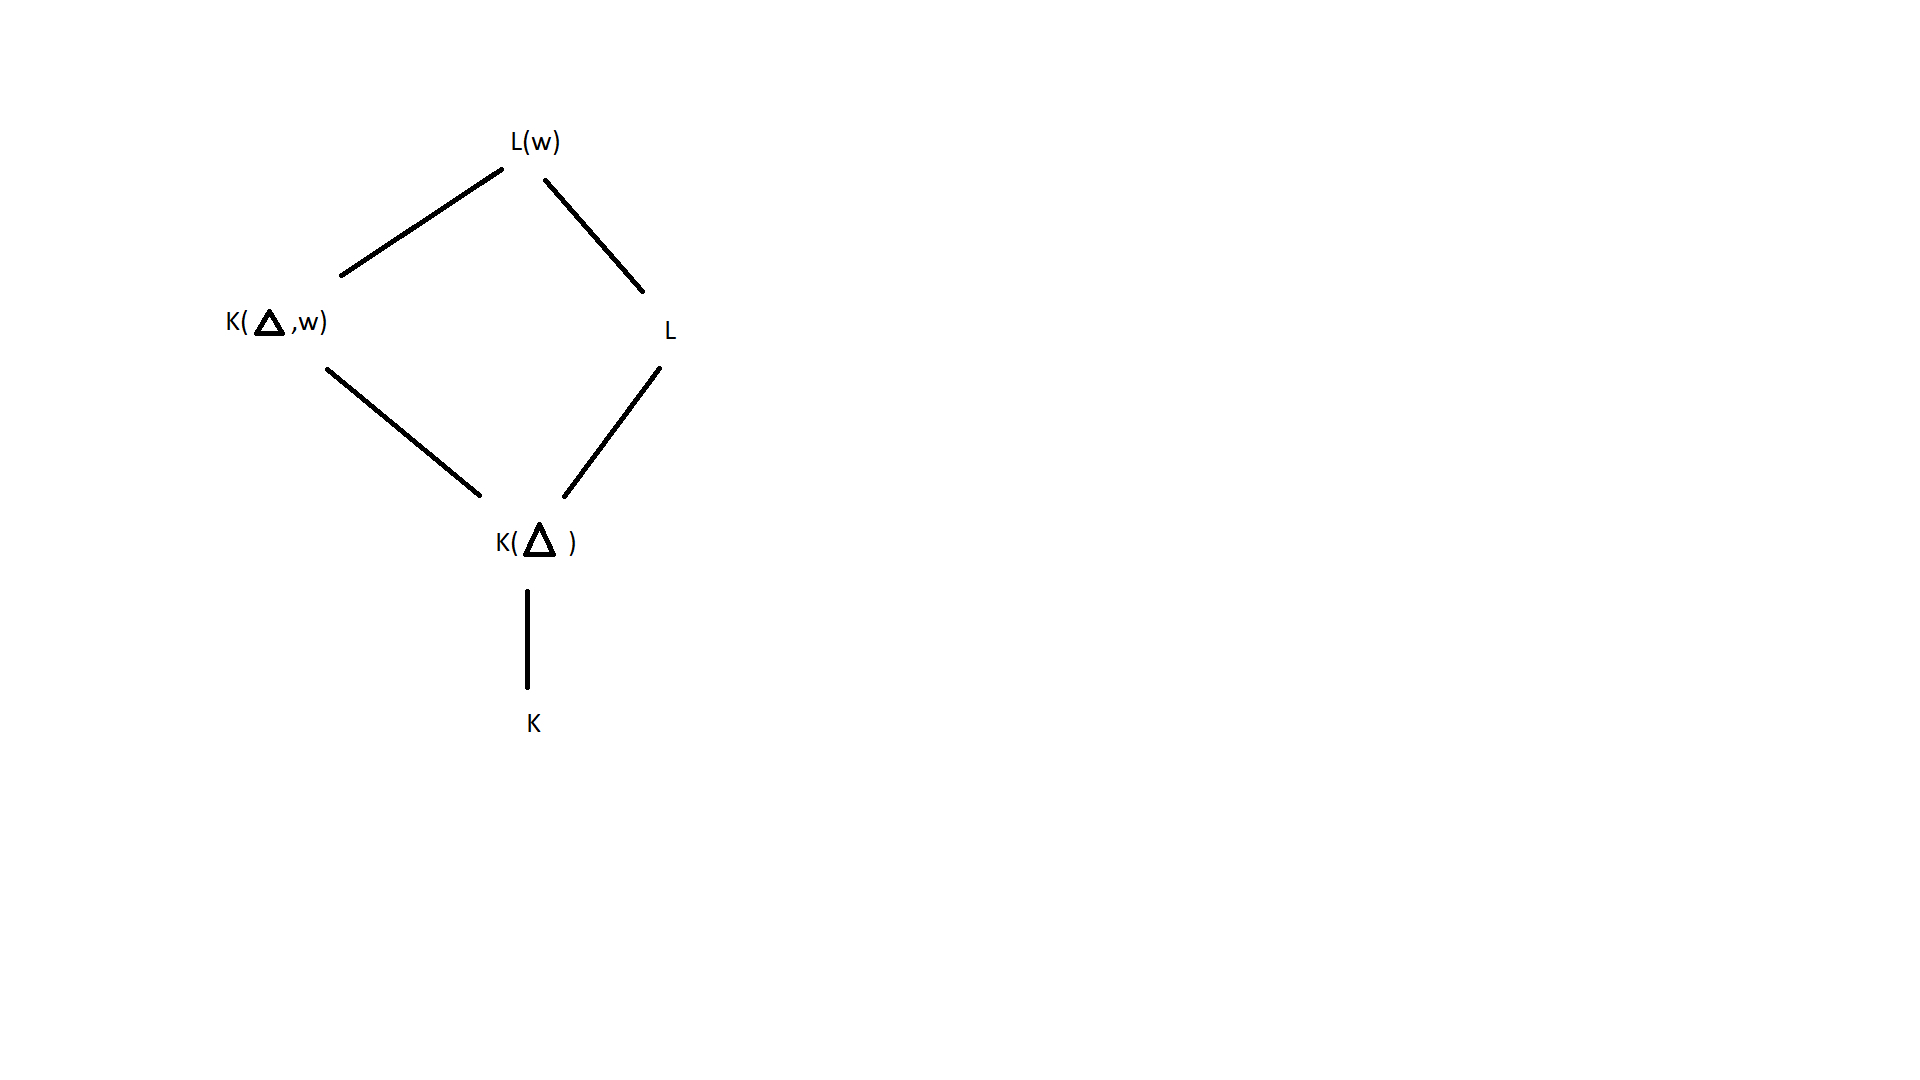
\includegraphics[scale=0.5]{image/GT_02.png}

From the tower law, $L(\omega):K(\Delta,\omega)| = 3$. Hence $\Gal(L(\omega)/K(\Delta,\omega)) \cong C_3$. We can apply (4.11) to see that $L(\omega) = K(\Delta,\omega) (\beta)$, where $\beta$ is a root of an irreducible polynomial $t^3-\lambda \in K(\Delta,\omega)[t]$. In fact, from the proof of (4.11) we see that $\beta = \alpha_1 + \omega\alpha_2+\omega^2\alpha_3$ where $\alpha_1,\alpha_2,\alpha_3$ are roots of $f(t)$. Now all the extensions $K \leq K(\Delta) \leq K(\Delta,\omega) \leq L(\omega)$ are cyclotomic or Kummer. So $f(t)$ is soluble by radicals.

In practice, Given irreducible cubic $f(t) = t^3+at^2+bt+c = (t-\alpha_1)(t-\alpha_2)(t-\alpha_3)$, we have $\alpha_1+\alpha_2+\alpha_3 = -a$. Replace $\alpha_i$'s by $\alpha_i' = \alpha_i + a/3$, so that $\alpha'_1+\alpha'_2+\alpha'_3 = 0$ and they are roots of a polynomial $g(t) = t^3+pt+q$, and $K(\alpha_1,\alpha_2,\alpha_3) = K(\alpha'_1,\alpha'_2,\alpha'_3$. Recall that the discriminant is $D(g) = -4p^3 - 27q^2$.

Set $\beta = \alpha'_1+\omega\alpha'_2+\omega^2\alpha'_3$, $\gamma = \alpha'_1+\omega^2\alpha'_2+\omega\alpha'_3$. Then 
\begin{equation*}
\begin{aligned}
\beta\gamma &= {\alpha'}_1^2+{\alpha'}_2^2+{\alpha'}_3^2 + (\omega+\omega^2)(\alpha'_1\alpha'_2+\alpha'_1\alpha'_3+\alpha'_2\alpha'_3)\\
&= (\alpha'_1+\alpha'_2+\alpha'_3)^2-3(\alpha'_1\alpha'_2+\alpha'_1\alpha'_3+\alpha'_2\alpha'_3)\\
&= -3p
\end{aligned}
\end{equation*}
and so $\beta^3\gamma^3 = -27p^3$. Now
\begin{equation*}
\begin{aligned}
\beta^3+\gamma^3 &=(\alpha_1+\omega\alpha'_2+\omega^2\alpha'_3)^3 + (\alpha'_1+\omega^2\alpha'_2+\omega\alpha'_3)^3 + (\alpha'_1+\alpha'_2+\alpha'_3)\\
&=3({\alpha'}_1^3+{\alpha'}_2^3+{\alpha'}_3^3) + 18\alpha'_1\alpha'_2\alpha'_3\\
&= -27q
\end{aligned}
\end{equation*}
since ${\alpha'}_1^3 = -p\alpha'_1-q$, and so ${\alpha'}_1^3+{\alpha'}_2^3+{\alpha'}_3^3 = -3q$. So $\beta^3$ and $\gamma^3$ are roots of a quadratic $t^2+27qt-27p^3$ and so are 
\begin{equation*}
\begin{aligned}
-\frac{27}{2}q \pm \frac{3\sqrt{-3}}{2} \sqrt{-27q^2-4p^3} = -\frac{27}{2}q \pm \frac{3\sqrt{-3}}{2} \sqrt{D}
\end{aligned}
\end{equation*}
We can solve for $\beta^3+\gamma^3$ in $K(\sqrt{-3},\sqrt{D}) = K(\omega,\Delta)$. We can get $\beta$ by adjoining a cube root of $\beta^3$, and then set $\gamma = -\frac{3p}{\beta}$. Finally we solve in $L(\omega)$ for $\alpha'_i$ to get
\begin{equation*}
\begin{aligned}
\alpha'_1 = \frac{1}{3}(\beta+\gamma),\\
\alpha'_2 = \frac{1}{3}(\omega^2\beta+\omega\gamma),\\
\alpha'_3 = \frac{1}{3}(\omega\beta+\omega^2\gamma)
\end{aligned}
\end{equation*}
(remember that $\alpha'_1+\alpha'_2+\alpha'_3 = 0$.)

\subsection{Quartics}
As with the cubics case, by making a substitution of the form $\alpha'_i = \alpha_i + a/4$, we may assume that the sum of the roots is zero, and so the $t^3$ term is zero. Then we have
\begin{equation*}
\begin{aligned}
f(t) = t^4+bt^2+ct+d = (t-\alpha_1)(t-\alpha_2)(t-\alpha_3)(t-\alpha_4)
\end{aligned}
\end{equation*}
monic irreducible. Let $L = K(\alpha_1,...,\alpha_4)$ be the splitting field for $f(t)$ over $K$. We have correspondence $L -- M =L^{G \cap V_4}$, normal extension of $K -- K(\Delta) -- K$ and $\{e\} -- G \cap V_4 \triangleleft G -- G\cap A_4 -- G = \Gal(L/K) \leq S_4$. By fundamental theorem $\Gal(M/K) \cong G/G\cap V_4$ by $\theta :S_4 \to S_3$, $\ker \theta = V_4$, $S_4/ V_4 \cong S_3$. $\theta|_G : G \to S_3$ satisfies $\ker \theta|_G = G\cap V_4$, $G/G\cap V_4 \cong im \theta|_G \leq S_3$. We therefore go looking for a cubic for which $M$ is the splitting field, called the resolvent cubic.

Now set $x = \alpha_1+\alpha_2$, $y=\alpha_1+\alpha_3$, $z=\alpha_1+\alpha_4$. We see that $\alpha_1 = \frac{1}{2}(x+y+z)$, $\alpha_2 = \frac{1}{2}(x-y-z)$, $\alpha_3 =\frac{1}{2}(-x+y-z)$, $\alpha_4 = \frac{1}{2}(-x-y+z)$. Thus $K(\alpha_1,...,\alpha_4) = K(x,y,z)$,
\begin{equation*}
\begin{aligned}
x^2 = (\alpha_1+\alpha_2)^2 = -(\alpha_1+\alpha_2)(\alpha_3+\alpha_4)\\
y^2 = (\alpha_1+\alpha_3)^2 = -(\alpha_1+\alpha_3)(\alpha_2+\alpha_4)\\
z^2 = (\alpha_1+\alpha_4)^2 = -(\alpha_1+\alpha_4)(\alpha_2+\alpha_3)
\end{aligned}
\end{equation*}
These are distinct e.g. if $y^2=z^2$ then $y = \pm z$, and so either $\alpha_3 = \alpha_4$ or $\alpha_1 = \alpha_2$. The $x^2,y^2,z^2$ are permuted by $G$ and are fixed by $G \cap V_4$. So $K(x^2,y^2,z^2) \leq M = L^{G \cap V_4}$. We claim that we have equality here, $M = K(x^2,y^2,z^2)$. Now consider the resolvent cubic $g(t) = (t-x^2)(t-y^2)(t-z^2) \in K[t]$. Note that its coefficients are fixed by $G$ and so lie in $K$.

To prove the claim, Observe that $D(f) = D(g)$ (example sheet), so $K(\Delta) \leq K(x^2,y^2,z^2)$. Now observe that $\Gal(L/K(x^2,y^2,z^2)) = \Gal(K(x,y,z)/K(x^2,y^2,z^2))$, $K(x^2,y^2,z^2) \leq K(x,y^2,z^2) \leq K(x,y,z^2) \leq K(x,y,z)$, where each extension is of degree 1 or 2. So $|K(x,y,z):K(x^2,y^2,z^2)|$ divides 8. So elements of $\Gal(L/K(x^2,y^2,z^2))$ have order dividing 8. But $\Gal(L/K(x^2,y^2,z^2)) \leq G \cap A_4$, so $\Gal(L/K(x^2,y^2,z^2)) \leq G \cap V_4$. Then by fundamental theorem we get $M = K(x^2,y^2,z^2)$.

Now consider the coefficients of $g(t)$: $x^2,y^2,z^2$ are permuted by $G$ and so the $g(t)$ are fixed by $G$ and therefore in $K$. $x^2+y^2+z^2 = -2b$, $x^2y^2+x^2z^2+y^2z^2 = b^2-4d$, $xyz = -c$ i.e. $x^2y^2z^2 = c^2$. So
\begin{equation*}
\begin{aligned}
g(t) = t^3 + 2bt^2 + (b^2-4d)t - c^2
\end{aligned}
\end{equation*}

We know how to solve cubics, so we can solve for $x^2,y^2,z^2$. Therefore we can solve for $x,y,z$. Then use our formulae from last time $\alpha_1 = \frac{1}{2}(x+y+z)$ etc.

\begin{rem}
Consider the map $\theta:S_4 \to S_3$, we have $\ker \theta = V_4$, $\theta|_{A_4}:A_4 \to A_3 \cong C_3$, $\theta|_{G \cap A_4} : G\cap A_4 \to A_3$, this has kernel $G \cap V_4$, so $G \cap A_4 / G \cap V_4 \cong $ subgroup of $A_3$. So we know $G\cap A_4$ has index 1 or 3 in $G \cap V_4$. So by correspondence, $L^{G \cap V_4}$ is an extension of order 1 or 3 over $K(\Delta)$. It is 3 if the resolvent cubic is irreducible, and is 1 if the cubic is reducible.
\end{rem}

For example, let $f(t) = t^4+4t^2+2$. We have $g(t) = t^3+8t^2+8t$ is reducible.

We are assuming $char K \neq 2$ from discussion about discriminants, and $char K \neq 3$ for cubic Kummer extensions.

\subsection{Solubility by radicals}
Now suppose we have a Galois extension $K \leq L$, with $K = L_0 \leq L_1 \leq ... \leq L_m = L$, such that $L_i \leq L_{i+1}$ is either cyclotomic or Kummer extension. Let $G = \Gal(L/K)$. There is a corresponding chain of subgroups of $G$, $G = G_0 \geq G_1 \geq ... \geq G_m = \{e\}$, with $G_i = \Gal(L/K_i)$, $L_i = L^{G_i}$ from Fundamental theorem. However, each extension $L_i \leq L_{i+1}$ is Galois, and we know $G_{i+1} = \Gal(L_i / L_{i+1}) \triangleleft \Gal(L/L_i) =  G_i$, and we know that the factor $G_i / G_{i+1} \cong \Gal(L_{i+1} / L_i)$, and RHS is abelian if $L_i \leq L_{i+1}$ is cyclotomic, and is cyclic if it's Kummer.

\begin{defi} (4.15)\\
A group is \emph{soluble} if there is a chain of subgroups $\{e\} = G_m \triangleleft G_{m-1} \triangleleft ... \triangleleft G_1 \triangleleft G_0 = G$ (*), with $G_i / G_{i+1}$ abelian.
\end{defi}

\begin{eg}
$S_3$ is soluble as $\{e\} \triangleleft <(123)> \triangleleft S_3$;\\
$S_4$ is soluble as $\{e\} \triangleleft V_4 \triangleleft A_4 \triangleleft S_4$, and $A_4/V_4 \cong C_3$, $S_4 / A_4 \cong C_2$.

Also, we know that $A_5$ is simple, and therefore any normal subgroup is either $\{e\}$ or $A_5$. As a result, any chain as in (*) in definition (4.15) would have non-abelian quotients. So $A_5$ is not soluble.
\end{eg}

\begin{lemma} (4.16)\\
A finite group $G$ is soluble if and only if we have $\{e\} = G_m \triangleleft G_{m-1} \triangleleft ... \triangleleft G_1 \triangleleft G_0 = G$ (**), with $G_i/G_{i+1}$ cyclic.
\begin{proof}
Backwards is definition. To show forward, we know about the structure of finite abelian groups. If $A$ abelian then there is a chain $\{e\} = A_4 \triangleleft A_{r-1} \triangleleft ... \triangleleft A_0 = A$ with $A_r /A_{r+1}$ cyclic. Thus we have a chain (*) with abelian factors $G_i / G_{i+1}$. But we can refine it (adding terms in between), to one of the form (**).
\end{proof}
\end{lemma}

\begin{defi} (4.17)\\
The \emph{derived subgroup} $G'$ of a group $G$ is the subgroup generated by all the commutators $g_1g_2g_1^{-1}g_2^{-1}$ for $g_1,g_2 \in G$.

Note that this is not necessarily a subgroup, so we'll have to check that.
\end{defi}

\begin{lemma} (4.18)\\
Let $K \triangleleft G$. Then $G/K$ abelian $\iff$ $G' \leq K$.
\begin{proof}
$G/K$ abelian $\iff$ $Kg_1 Kg_2 Kg_1^{-1} Kg_2^{-1} = K$ for all $g_1,g_2 \in G$ $\iff$ $g_1g_2g_1^{-1} g_2^{-1} \in K$ $\iff G' \leq K$.
\end{proof}
\end{lemma}

\begin{rem}
$\bullet$ Next etrm in representation theory we'll prove Burnside's theorem: If $|G| = p^a q^b$, $p,q$ distinct primes, then $G$ is soluble.\\
$\bullet$ Also Feit-Thompson theorem: if $|G|$ is odd, then $G$ is soluble.\\
$\bullet$ There's an analogue of Sylow's theorems due to Philip Hall: for all $|G| = mn$, with $(m,n)$ coprime, there is a subgroup of order $m$ if and only if $G$ is soluble.
\end{rem}

\begin{defi} (4.19)\\
The derived series $\{G^{(m)}\}$ of $G$ is defined inductively: $G^{(0)} =G, G^{(1)} = G',G^{(2)} = (G')'$,...

Thus we have

\begin{equation*}
\begin{aligned}
G = G^{(0)} \triangleright G^{(1)} \triangleright ...
\end{aligned}
\end{equation*}
with $G^{(j)} / G^{(j+1)}$ abelian.
\end{defi}

\begin{lemma} (4.20, for $G$ finite)\\
$G$ is soluble iff $G^{(m)} = \{e\}$ for some $m$.
\begin{proof}
If $G^{(m)} = \{e\}$, then the derived series gives a chain of the form (*) (in 4.15) in the definition of solubility.

Conversely, if there is a chain of the form (*), $G \triangleright G_1 \triangleright G_2 \triangleright ... \triangleright G_m = \{e\}$, with $G_i / G_{i+1}$ abelian, then an easy induction shows that $G^{(j)} \leq G_j$, and so $G^{(m)} = \{e\}$.
\end{proof}
\end{lemma}

\begin{rem}
The derived series is the fastest descending chain with abelian factors.
\end{rem}

\begin{lemma} (4.21)\\
(i) Let $H \leq G$, $G$ soluble, then $H$ is soluble.\\
(ii) Let $H \triangleleft G$, then $G$ soluble $\iff$ $H$ and $G/H$ are both soluble.
\begin{proof}
(i) $G$ soluble $\implies$ $G^{(m)} = \{e\}$ by (4.20). But $H^{(m)} \leq G^{(m)}$, so $H$ is soluble by 4.20.\\
(ii) Let $H \triangleleft G$. Then $G$ soluble $\implies$ $H$ soluble by (i).\\
$G$ soluble $\implies$ $G^{(m)} = \{e\}$ say. Observer that $(G/H)' = G'H/H \leq GH$, similarly $(G/H)^{(j)} = G^{(j)} H/H \leq G/H$, thus $(G/H)^{(m)} = H/H$ trivial subgroup of $G/H$, and so $G/H$ is soluble.

Now consider the converse. Suppose that $H$ and $G/H$ are soluble. Then $H^{(r)} = \{e\}$ and $(G/H)^{(s)} = H/H$ for some $r,s$. But then $(G/H)^{(s)} = G^{(s)} H/H$, so $G^{(s)} H \cong H$ and thus $G^{(s)} \leq H$. Hence $G^{(r+s)} \leq H^{(r)} = \{e\}$. Thus $G$ is soluble.
\end{proof}
\end{lemma}

\begin{eg}
$S_5$ is not soluble, since its subgroup $A_5$ is not soluble.
\end{eg}

\begin{thm} (4.22)\\
Let $K$ be a field, and $f(t) \in K[t]$. Assume $char K = 0$. Then $f(t)$ is soluble by radicals over $K$ $\iff$ $\Gal(f)$ over $K$ is soluble.
\begin{rem}
We don't need to restrict to $charK = 0$. What we need to do for a particular $f(t)$ is to avoid a finite number of bad characteristics (avoid characteristics $\leq \deg f(t)$).
\end{rem}
\end{thm}

\begin{coro} (4.23)\\
If $f(t)$ is a monic irreducible polynomial in $K[t]$ with $\Gal(f) \cong A_5$ or $S_5$, then $f(t)$ is not soluble by radicals (with $char K = 0$).
\end{coro}

\begin{eg}
In example 3.9(i), we had $f(t) = t^t-6t+3 \in \Q[t]$, and we've seen that $\Gal(f)$ over $\Q$ is $S_5$ (recall we had 3 real roots and complex conjugation gives a transposition, $f(t)$ is irreducible and so $5|\Gal(f)$, so we've also got a 5-cycle and these generate $S_5$). So $f(t)$ is not soluble by radicals.
\end{eg}

\begin{proof} (of 4.22)\\
Suppose $f(t)$ is soluble by radicals. Thus if $L$ is the splitting field of $f(t)$ over $K$, then $L$ lies in an extension of $K$ by radicals $K = L_0 \leq L_1 \leq ... \leq L_m$ with each $L_i \leq L_{i+1}$ is cyclotomic or Kummer. At this stage we don't know that $L_m$ is Galois over $K$. At this stage, we don't know that $L_m$ is Galois over $K$. So we'll need something else first:

\begin{lemma} (4.24)\\
If $K \leq N$ is an extension by radicals, then $\exists N'$ with $N \leq N'$, $K \leq N'$ is an extension of radicals, and $K \leq N'$ being a Galois extension.
\end{lemma}

Assuming this lemma, and so we may assume that $L_m$ is Galois over $K$. Then by Fundamental theorem of Galois Theory (3.2), there is a corresponding chain of subgroups of $\Gal(L_m/K)$. Our previous discussion at the beginning of this section (before (4.13)) we know that $\Gal(L_m / K)$ is soluble, because our chain has abelian factors. But $K \leq L \leq L_m$ with $K \leq L$ Galois, by the Fundamental theorem (3.2(iii)), the Galois group $\Gal(L/K) \cong \Gal(L_m/K)/\Gal(L_m/L)$. But quotients of soluble groups are soluble. So $\Gal(L/K)$ is soluble.
\end{proof}

\begin{proof} (of 4.24)\\
We have $K=L_0 \leq L_1 \leq ... \leq L_m$, with each $L_i \leq L_{i+1}$ cyclotomic or Kummer, and we want to embed this into a Galois extension of the same form. Assume $char K = 0$. By the primitive elemnt theorem, $L_m = K(\alpha_1)$ for some $\alpha_1$.\\
Let $g(t)$ be the minimal polynomial of $\alpha_1$ over $K$, with splitting field $M$. Thus $M = K(\alpha_1,...,\alpha_n)$ where $\alpha_i$ are roots of $g(t)$. There are $K$-homomorphisms $\phi_1:M \to M$ by $\alpha_1 \to \alpha_i$, extending the $K$-homomorphisms $K(\alpha_1) \to K(\alpha_i) \leq M$. The tower $K \leq \phi_i(K) \leq \phi_i(L_1) \leq ... \leq \phi_i(L_m) = K(\alpha_i)$, with cyclotomic or Kummer extensions as before.\\
Consider $$L_m = K(\alpha_1) \leq \phi_2(L_1)(\alpha_1) \leq \phi_2(L_2)(\alpha_1) \leq ... \leq \phi_2(L_m)(\alpha_1) = K(\alpha_1,\alpha_2)$$\\
Consider the extension $\phi_2(L_j)(\alpha_1) \leq \phi_2(L_{j+1})(\alpha_1)$: if $L_j \leq L_{j+1}$ cyclotomic, then all the roots of unity adjoined are now in $L_m = K(\alpha_1)$ and so $\phi_2(L_j)(\alpha_1) = \phi_2(L_{j+1})(\alpha_1)$. If $L_j \leq L_{j+1}$ then we obtain $L_{j+1}$ by adjoining roots of an element of $L_j$, and so we obtain $\phi_2(L_{j+1})$ by adjoining roots of an element in $\phi_2(L_j)$. Hence we get from $\phi_2(L_j)(\alpha_1)$ to $\phi_2(L_{j+1})(\alpha_1)$ by adjoining roots of an element of $\phi_2(L_j)$. So it's a Kummer extension.\\
Now continue to get a suitable chain $K(\alpha_1,\alpha_2) \leq ... \leq K(\alpha_1,\alpha_2,\alpha_3)$ etc. Thus we get a suitable chain from $K$ to $K(\alpha_1,...,\alpha_n) = M$. Observe that $K \leq M$ is Galois.
\end{proof}

Converse of (4.22): Suppose $G = \Gal(f)$ over $K$ is soluble. Let $L$ be the splitting field of $f(t)$ over $K$ and so $|G| = |L:k| =n$. Set $m=n!$, and let $\xi$ be a primitive $m$th root of unity and consider $L(\xi)$. Our proof is similar to that used for cubics.\\
Observe that $|L(\xi):K(\xi)| \leq n$: by primitive element theorem $L=K(\alpha)$ for some $\alpha$ with minimal polynomial $g(t)$ say of degree $n$. Then $L(\xi) = K(\xi)(\alpha)$, and the minimal polynomial of $\alpha$ over $K(\xi)$ divides $g(t)$, so is of degree $\leq n$. Note that $\Gal(L(\xi)/L)$ is abelian, since the extension is cyclotomic. Then $\Gal(L(\xi)/K)$ is soluble since $\Gal(L(\xi) / L)$ soluble and $\Gal(L/K) \cong \Gal(L(\xi)/K) / \Gal(L(\xi)/L)$ soluble by Fundamental theorem and (4.21). Then the subgroup $\Gal(L(\xi)/K(\xi)) \leq \Gal(L(\xi)/K)$ is soluble by (4.21). Thus there is a chain of subgroups $\Gal(L(\xi)/K(\xi)) = G_0 \triangleright G_1 \triangleright ... \triangleright G_m = \{e\}$, with $G_i/G_{i+1}$ cyclic (using (4.16)). Now use the Fundamental theorem to get a corresponding chain of fields $k9\xi) \leq K_1 \leq ... \leq K_m = L(\xi)$ with each $K_i \leq K_{i+1}$ Galois, with cyclic Galois group.\\
Theorem (4.11) now says that all those extensions are Kummer (note all the extensions are of degree $\leq n$, and so we have the appropriate roots of unity). Thus we've embedded $L$ in an extension of $K$ by radicals.

\begin{eg}
$f(t) = t^4+4t^2+2$. This is irreducible over $\Q$ by Eisenstein. Resolvent cubic $g(t) = t^3+8t^2+8t$, its roots are 0 and $-4 \pm 2\sqrt{2}$, so its splitting field $L$ has degree 8 over $K=\Q$, and is degree 4 over $K(\sqrt{2})$. The Galois group is transitive of degree 8 in $S_4$, so must be $D_8$.
\end{eg}

\begin{eg}
$f(t) = t^4+2t+2$ over $\Q$, which is irreducible by Eisenstein. Its discriminant is $101 \cdot 4^2$ which is not a square. The resolvent cubic $g(t) = t^3-8t-4$ is irreducible (as it's irreducible mod 5). So $\Gal(f)$ is transitive, but not in $A_4$, and has a 3-cycle. So $\Gal(f) = S_4$.
\end{eg}

\begin{eg}
$f(t) = t^5-t-1$ is also irreducible over $\Q$ since it's irreducible mod 5. So its Galois group contains a 5-cycle and is transitive. Consider mod 2, $f$ factorises as a product of irreducible cubic and irreducible quadratic $(t^3+t^2+1)(t^2+t+1)$. So $\Gal(\bar{f})$ generated by an element of cycle type 3,2. So $\Gal(f)$ also contains an element of cycle type 3,2. Then $g^3$ is a transposition. Therefore $\Gal(f) = S_5$ Then $g^3$ is a transposition. Therefore $\Gal(f) = S_5$ over $\Q$.
\end{eg}

\newpage

\section{Final Thoguhts}
\subsection{Algebraic Closure}
\begin{defi}(5.1)\\
A field $L$ is \emph{algebraically closed} if any $f(t) \in L[t]$ splits into a product of linear factors in $L[t]$.
\end{defi}

\begin{rem}
This is equivalent to saying that any $f(t) \in L[t]$ has a root in $L$ \emph{or} that any algebraic extension of $L$ is $L$ itself.
\end{rem}

\begin{defi}(5.2)\\
An extension $K \leq L$ is an \emph{algebraic closure} of $K$ if $K \leq L$ is algebraic and $L$ is algebraically closed.
\end{defi}

\begin{lemma}(5.3)\\
If $K \leq L$ is algebraic and every polynomial in $K[t]$ splits completely over $L$ then $L$ is an algebraic closure of $K$.
\begin{proof}
We need to show $L$ is algebraically closed. Suppose $L \leq L(x)$ is a finite extension, and $f_\alpha(t) = t^n+a_{n-1}t^{n-1}+...+a_0$ is the minimal polynomial of $\alpha$ over $L$. Let $M = K(\alpha_0,...,\alpha_{n-1}$. Then $M \leq M(\alpha)$ is a finite extension. But each $a_i$ is algebraic over $K$ and so $|M:K|<\infty$. Hence $|M(\alpha):K|<\infty$ by Tower Law, and so $\alpha$ is algebraic over $K$.

The minimal polynomial of $\alpha$ over $K$ must split over $L$, and so $\alpha \in L$. Thus any algebraic extension of $L$ is $L$ itself.
\end{proof}

\begin{eg}
$\mathbb{A} = \{\alpha \in \C:\alpha$ algebraic over $\Q\}$. It is a subfield of $\C$: if $\alpha,\beta$ are algebraic over $\Q$, then $|\Q(\alpha,\beta):\Q|<\infty$, so if $\gamma = \alpha+\beta,\alpha-\beta,\alpha\beta$ or $\alpha/\beta \neq 0$, we get $\Q(\gamma) \leq \Q(\alpha,\beta)$ and so $|\Q(\gamma):\Q| < \infty$. So $\gamma$ is algebraic over $\Q$, and so $\gamma \in \mathbb{A}$. Therefore $\mathbb{A} = \bar{\Q}$ is an algebraic closure of $\Q$.
\end{eg}
\end{lemma}

However, if we want to prove existence and uniqueness of algebraic closures in general, then we need to appeal to Zorn's lemma (see Logic and Set Theory), and it's equivalent to the Axiom of Choice and the Well-Ordering Principle.

\begin{defi}
$(\mathcal{S},\leq)$ is a partial order on $\mathcal{S}$ if:\\
(i) $x \leq x$ $\forall x \in \mathcal{S}$;\\
(ii) $x \leq y$ and $y \leq z$ $\implies x \leq z$;\\
(iii) if $x \leq y$ and $y \leq x$ then $x = y$.
\end{defi}

$\mathcal{S}$ is \emph{totally ordered} if for any $x,y \in \mathcal{S}$, either $x \leq y$ or $y \leq x$.

A \emph{chain} in a partially ordered set $(\mathcal{S},\leq)$ is a totally ordered subset.

\begin{lemma} (5.5, Zorn's Lemma (actually an axiom))\\
If $(\mathcal{S},\leq)$ be a non-empty partially ordered set. Suppose that any chain has an upper bound in $\mathcal{S}$(?). Then $\mathcal{S}$ has a maximal element.
\end{lemma}

\begin{lemma} (5.6)\\
Let $R$ be a non-trivial ring with multiplicative unity. Then $R$ has a maximal ideal.
\begin{proof}
Let $\mathcal{S}$ be the set of proper ideals of $R$, so this is non-empty since $(0)$ is proper as $R$ is non-trivial. We partially order $\mathcal{S}$ by inclusion. We know any ideal $I$ is proper $\iff$ $1 \not\in I$. Any chain of proper ideals has an upper bound in $\mathcal{S}$, namely the union of chain. Then apply Zorn's lemma we know $\mathcal{S}$ has a maximal element, i.e. a maximal ideal of $\R$.
\end{proof}
\end{lemma}

\begin{thm} (5.7, existence of algebraic closures)\\
For any field $K$, there is an algebraic closure.
\begin{proof}
Let $\mathcal{S} = \{(f(t),j)$ $f(t)$ irreducible monic in $K[t]$, $1 \leq j \leq \deg f\}$. For each pair $s=(f(t),j)$, we introduce an indeterminate $X_s = X_{f,j}$. Consider the polynomial ring $K[X_s, s \in \mathcal{S}]$, and set $\tilde{f}(t) = f(t) - \prod_{i=1}^{\deg f} (t-X_{f,j}) \in K[X_s, s \in \mathcal{S}][t]$. Let $I \triangleleft K[X_s, s \in \mathcal{S}]$ generated by all the coefficients of all the $\tilde{f} (t)$. Denote the coefficients of $\tilde{f}(t)$ by $a_{f,l}$ for $0 \leq l \leq \deg{f}$. We claim that $I \neq K[X_s, s \in \mathcal{S}]$.\\
To prove that, suppose $1 \in I$ and we try to get a contradiction. We have $b_1 a_{f_1,l_1}+...+b_n a_{f_N,l_N} = 1$ in $K[X_s, s \in \mathcal{S}]$ (+). Let $L$ be a splitting field for $f_1(t)...f_N(t)$ (product). For each $i$, $f_i$ splits over $L$. So $f_i(t) = \prod_{j=1}^{\deg f_i} (t-\alpha_{ij}$. Define a $K$-linear ring homomorphism, which is identity on $K$: $\theta$: $K[X_s, s \in \mathcal{S}] \to L$ by $X_{f_i,j} \to \alpha_{i,j}$, $X_s \to 0$ otherwise. This induces a map $K[X_s,s \in \mathcal{S}] \to L[t]$. Then $\theta(\tilde{f}_i(t)) =\theta(f_i(t)) - \prod_{j=1}^{\deg f_i} \theta(t-X_{f_i,j}) = f_i(t) - \prod_{j=1}^{\deg f_i} (t-\alpha_{i,j}) = 0$. But then $\theta(a_{f_i,j}) = 0$ since $a_{f_i,j}$ are the coefficients of $\tilde{f}_i(t)$. But applying $\theta$ to (+) we get $0=1$. Contradiction.
Then $I$ is a proper ideal of $K[X_s,s \in \mathcal{S}]$. By Zorn's lemma there is a maximal ideal $P$ of $K[X_s,s \in \mathcal{S}]$ containing $I$. set $L_1 = K[X_s,s \in \mathcal{S}] / P$ a field. Thus we have a field extension $K \leq L_1$. We claim that $L_1$ is an algebraic closure of $K$.\\
We now prove that $K \leq L_1$ is algebraic. $L_1$ is generated by the images $x_{f,j}$ of the $X_{f,j}$. However $\tilde{f}(j)$ has coefficients in $I$ and so its image in $L_1[t]$ is the zero polynomial. Thus in $L_1[t]$, $f(t) = \prod (t-x_{f,j})$ (*), and so $f(x_{f,j}) = 0$. Thus the $x_{f,j}$ are algebraic. Any element of $L_1$ involves only finitely many of the $x_{f,j}$, and so is algebraic over $K$. Moreover, from (*), any $f(t) \in K[t]$ splits completely over $L_1$. The theorem follows from (5.3).
\end{proof}
\end{thm}

\begin{thm} (5.8)\\
Suppose $\theta:K \to L$ is a ring homomorphism and $L$ is algebraically closed. Suppose $K \leq M$ is an algebraic extension. Then $\theta$ can be extended to a homomorphism $\phi:M \to L$ (i.e. $\phi|_K = \theta$).
\begin{proof}
Let $\mathcal{S} = \{(N,\phi):K \leq N \leq M, \phi$ homomorphism $N \to L$ extending $\theta\}$. Partially order $\mathcal{S}$ by $(N_1,\phi_1) \leq (N_2,\phi_2)$ if $N_1 \leq N_2$ and $\phi_2|_{N_1} = \phi_1$. $\mathcal{S}$ is non-empty since $(K,\theta) \in \mathcal{S}$. Now if there is a chain $(N_1,\phi_1) \leq ...$ then set $N = \bigcap N_\lambda$. This is a subfield of $M$, and we can define $\chi:N \to L$ as follows: if $\alpha \in N$ then $\alpha \in N_\lambda$ for some $\lambda$ and we set $\psi(\alpha) = \phi_\lambda(\alpha)$. This is well defined. Thus $(N,\psi)$ is an upper bound for our chain in $\mathcal{S}$. Zorn applies to give a maximal element of $\mathcal{S}$ $(N,\phi)$. We now show $N = M$. Given $\alpha \in M$, it's algebraic over $K$, and hence over $N$. Let $F_\alpha(t)$ be its minimal polynomial over $N$. But $\phi f(t)$ is in $L[t]$ and so splits completely over $L$, since $L$ algebraically closed. So $\phi f(t) = (t-\beta_1)...(t-\beta_r)$ say. Since $\phi f(\beta_j) = 0$, there is a map $N(\alpha) \cong N[t] / (f_\alpha(t)) \to L$ by $\alpha \to \beta_1$ extending $\phi$. Maximality of $(N,\phi)$ implies that $N(\alpha) = N$. So $\alpha \in N$. Thus $N=M$.
\end{proof}
\end{thm}

\begin{thm} (5.9, uniqueness of algebraic closure)\\
If $K \leq L_1$, $K \leq L_2$ are two algebraic closures of $K$, then there exists an isomorphism $\phi$:$L_1 \to L_2$.
\begin{proof}
By (5.8) there is a homomorphism $\phi:L_1 \to L_2$ extending the embedding $K$ in $L_2$. Since $K \leq L_2$ is algebraic, so also is $K \leq \phi(L_1)$. But $L_1$ is algebraically closed and so $\phi(L_1)$ is algebraicaly closed. So $L_2 = \phi(L_1)$ and $\phi$ is an isomorphism.
\end{proof}
\end{thm}

\subsection{Symmetric polynomials and invariant theory}
In the build up of the Fundamental Theorem we met Artin's Theorem (3.3). Let $K \leq L$ and $H$ finite subgroup of $\Aut_K(L)$. Let $M = L^H$. Then $M \leq L$ is a Galois extension and $H = \Gal(L/M)$.

\begin{eg}
$L = K(X_1,...,X_n)$. Let $S_n$ permute the variables. These permutations induce $K$-automorphisms of $L$. By Artin's theorem, if $M = L^{S_n} \leq L$ then it is Galois and $\Gal(L/M) = S_n$. Thus $S_n$ is aGalois group of some field extension. We know that we can regard any finite group $G$ as a subgroup of some $S_n$ and so we see that any finite group is a Galois group of some field extension (using Fundamental Theorem).

Now consider $f(t) = (t-X_1)...(t-X_n) \in M[t] = t^n - s_1 t^{n-1} + ... + (-1)^n s_n$. Thus $s_1 = X_1 + ... +X_n,...,s_n = X_1...X_n$.
\end{eg}

\begin{defi} (5.10)\\
These $s_i$ are the \emph{elementary symmetric polynomials}.
\end{defi}

\begin{thm} (5.11)\\
The fixed field $M=L^{S_n} = K(s_1,...,s_n)$ and the $s_1,...,s_n$ are algebraically indepndent over $K$ (in $L$).
\end{thm}

\begin{defi} (5.12)\\
$\alpha_1,...,\alpha_n$ are algebraically independent over $K$ if the ring homomorphism $K[Y_1,...,Y_n] \to K[\alpha_1,...,\alpha_n] \leq L$ is an isomorphism, where $K[Y_1,...,Y_n]$ is the polynomial ring in $Y_1,...,Y_n$.
\end{defi}


\end{document}
